\documentclass{article}
\usepackage{graphicx}
\usepackage{appendix}
\usepackage{url}
\usepackage[margin=3.3cm]{geometry}
\usepackage{subcaption}
\usepackage{hyperref}
\hypersetup{pdfborder={0 0 0}}

\title{Can Masked Self-Supervised Learning improve the Robustness of budget limited Keypoint based Sign Language Recognition}
\author{Will Pitt - xe25973 \\ 
        Supervised by: Dr. Qianhui Men}

\begin{document}
\maketitle

\begin{abstract}
Keypoint based Sign Language Recognition (SLR) is a cheap viable alternative to video based models, reaching state of the art Sign Language Translation quality. Keypoint models are trained using keypoint datasets generated by processing video with pose estimators. This however leaves the models vulnerable to errors baked into the keypoint datasets, due to pose estimator failures and corruptions in the video stream such as fast movements and obstruction of body parts. Self-Supervised Learning (SSL) has proven performance improvements in language related tasks but has seen limited study for keypoint based SLR. 

The aim of this study is to identify whether the robustness and accuracy of an existing keypoint SLR model can be improved with SSL with a limited compute budget. SSL was performed with corruptions simulating pose estimator failures and validated with a probe before being fine tuned and analysed with a robustness suite. 

The SSL produced no statistically significant improvement in accuracy or robustness but did reshape the robustness of the model. This was likely due to the objective of the SSL not aligning with gloss discriminative objectives. 

Reconstruction based masked SSL did not improve keypoint SLR. Therefore further work investigating the effect of discriminative SSL should be recommended.

\vspace{35mm} 
\end{abstract}

\textbf{Ethics statement: } 
This project fits within the scope of ethics application 15208, as reviewed by my supervisor, Qianhui Men. I have completed the ethics test on Blackboard. My score is 12/12.

\newpage % END THE TITLE PAGE
\tableofcontents

\newpage

\section{Introduction}

\subsection{Sign Language Overview}
Sign languages are visual languages, communicated by performing manual movements and non-manual expressions. The languages have developed as part of communities of deaf people within different countries and form a large part of deaf culture within that country. Sign languages are not universal and with no direct one to one mapping to a spoken language, with American Sign Language (ASL) and British Sign Language (BSL) being spoken in many countries with the shared English language. In sign language, manual gestures are performed to mean different concepts. Each sign may be accompanied by mouth movement, facial expressions and changes of gaze or body position. The signs may not be in the order of the equivalent words used in a spoken language and there is no grammar or punctuation to specify when a sentence has ended \cite{el-alfy_comprehensive_2022} \cite{camgoz_neural_2018}. There are cultural differences between these languages, such as BSL often having signers mouth the word being signed \cite{vedaldi_bsl-1k_2020}. There are commonalities between the gestures used in sign languages, but a universal sign language has seen little adoption outside of international conferences. There is opposition to adoption of a universal sign language within deaf communities due to the risk of eroding the rich culture connected to localised sign language.\cite{bragg_sign_2019}

\subsection{Sign Language Translation difficulties}
Sign Language Recognition (SLR) is the act of identifying the signs which are performed, the notation of the signs in this form are known as a gloss. For example the sentence "I was born in London" may be represented in BSL by the gloss "me born where? London". Sign language Translation (SLT) involves both identifying the signs and translating them into a natural language. Models which translate signs may be directly translated to natural language (Sign2Text) or via an intermediate step of gloss which can be trained (Sign2Gloss2Text) \cite{zhou_gloss-free_2023}. One difficulty of SLT is how signs may appear across multiple, unaligned channels simultaneously. Facial express, mouthing and each hand position may all contribute to the meaning of the sign and these may not all align perfectly to the same time period \cite{el-alfy_comprehensive_2022}.
Another difficulty of SLT is how there are limited datasets with expertly labelled translations for both gloss and text, limiting supervised learning for SLR. Phoenix2014T, which is often used to benchmark model performance, contains around 8000 examples from 9 signers and every signer appears in every split of the data. Phoenix2014T is produced by a German weather channel and so the subject and vocabulary is limited. 
A further difficulty relates to how there may be multiple methods of signing the same meaning within a sign language. Different signers may cause variance in a dataset due to different sign preferences, skin tone, body size and clothing. 

\subsection{Keypoint encoding is well suited to SLT and SLR} 
Multi-Stream Keypoint Attention network (MSKA \cite{guan_multi-stream_2024}) is an existing high performance model which uses keypoints generated by an independent pose estimator for SLR and SLT. Keypoints are a coordinate system of body markers which represent landmarks and joints on a human body. Keypoints can be used as an alternative or alongside a video feed to identify signs as part of SLT. Keypoint models have been shown to maintain high performance whilst requiring far smaller models and computer time when compared to video.  Keypoints also benefit by being less affected by the signers clothing and skin colour allowing models to generalise better to unseen signers \cite{min_closer_2025}. However errors may be generated during keypoint capture due to motion blur, hand obstruction and other artefacts. Each keypoint captured is given a confidence score, which is fed into the model allowing it to factor this confidence in the predictions. Figure \ref{fig:HRNet_confidence} shows the distribution of the confidence of the HRNet model for different body part keypoints. The face is always well lit and facing the camera and so is largely well seen. The hands are often well captured but have moments where they are moving quickly resulting in some moments of low confidence. It is worth noting that during signing, the non-dominant left hand is more likely to be obscured or out of shot and so it has more instances of low confidence \cite{el-alfy_comprehensive_2022}. The body is never recorded below the waist and so the graph is showing examples of inaccuracy in the model where it is hallucinating feet.

\begin{figure}[htbp]
  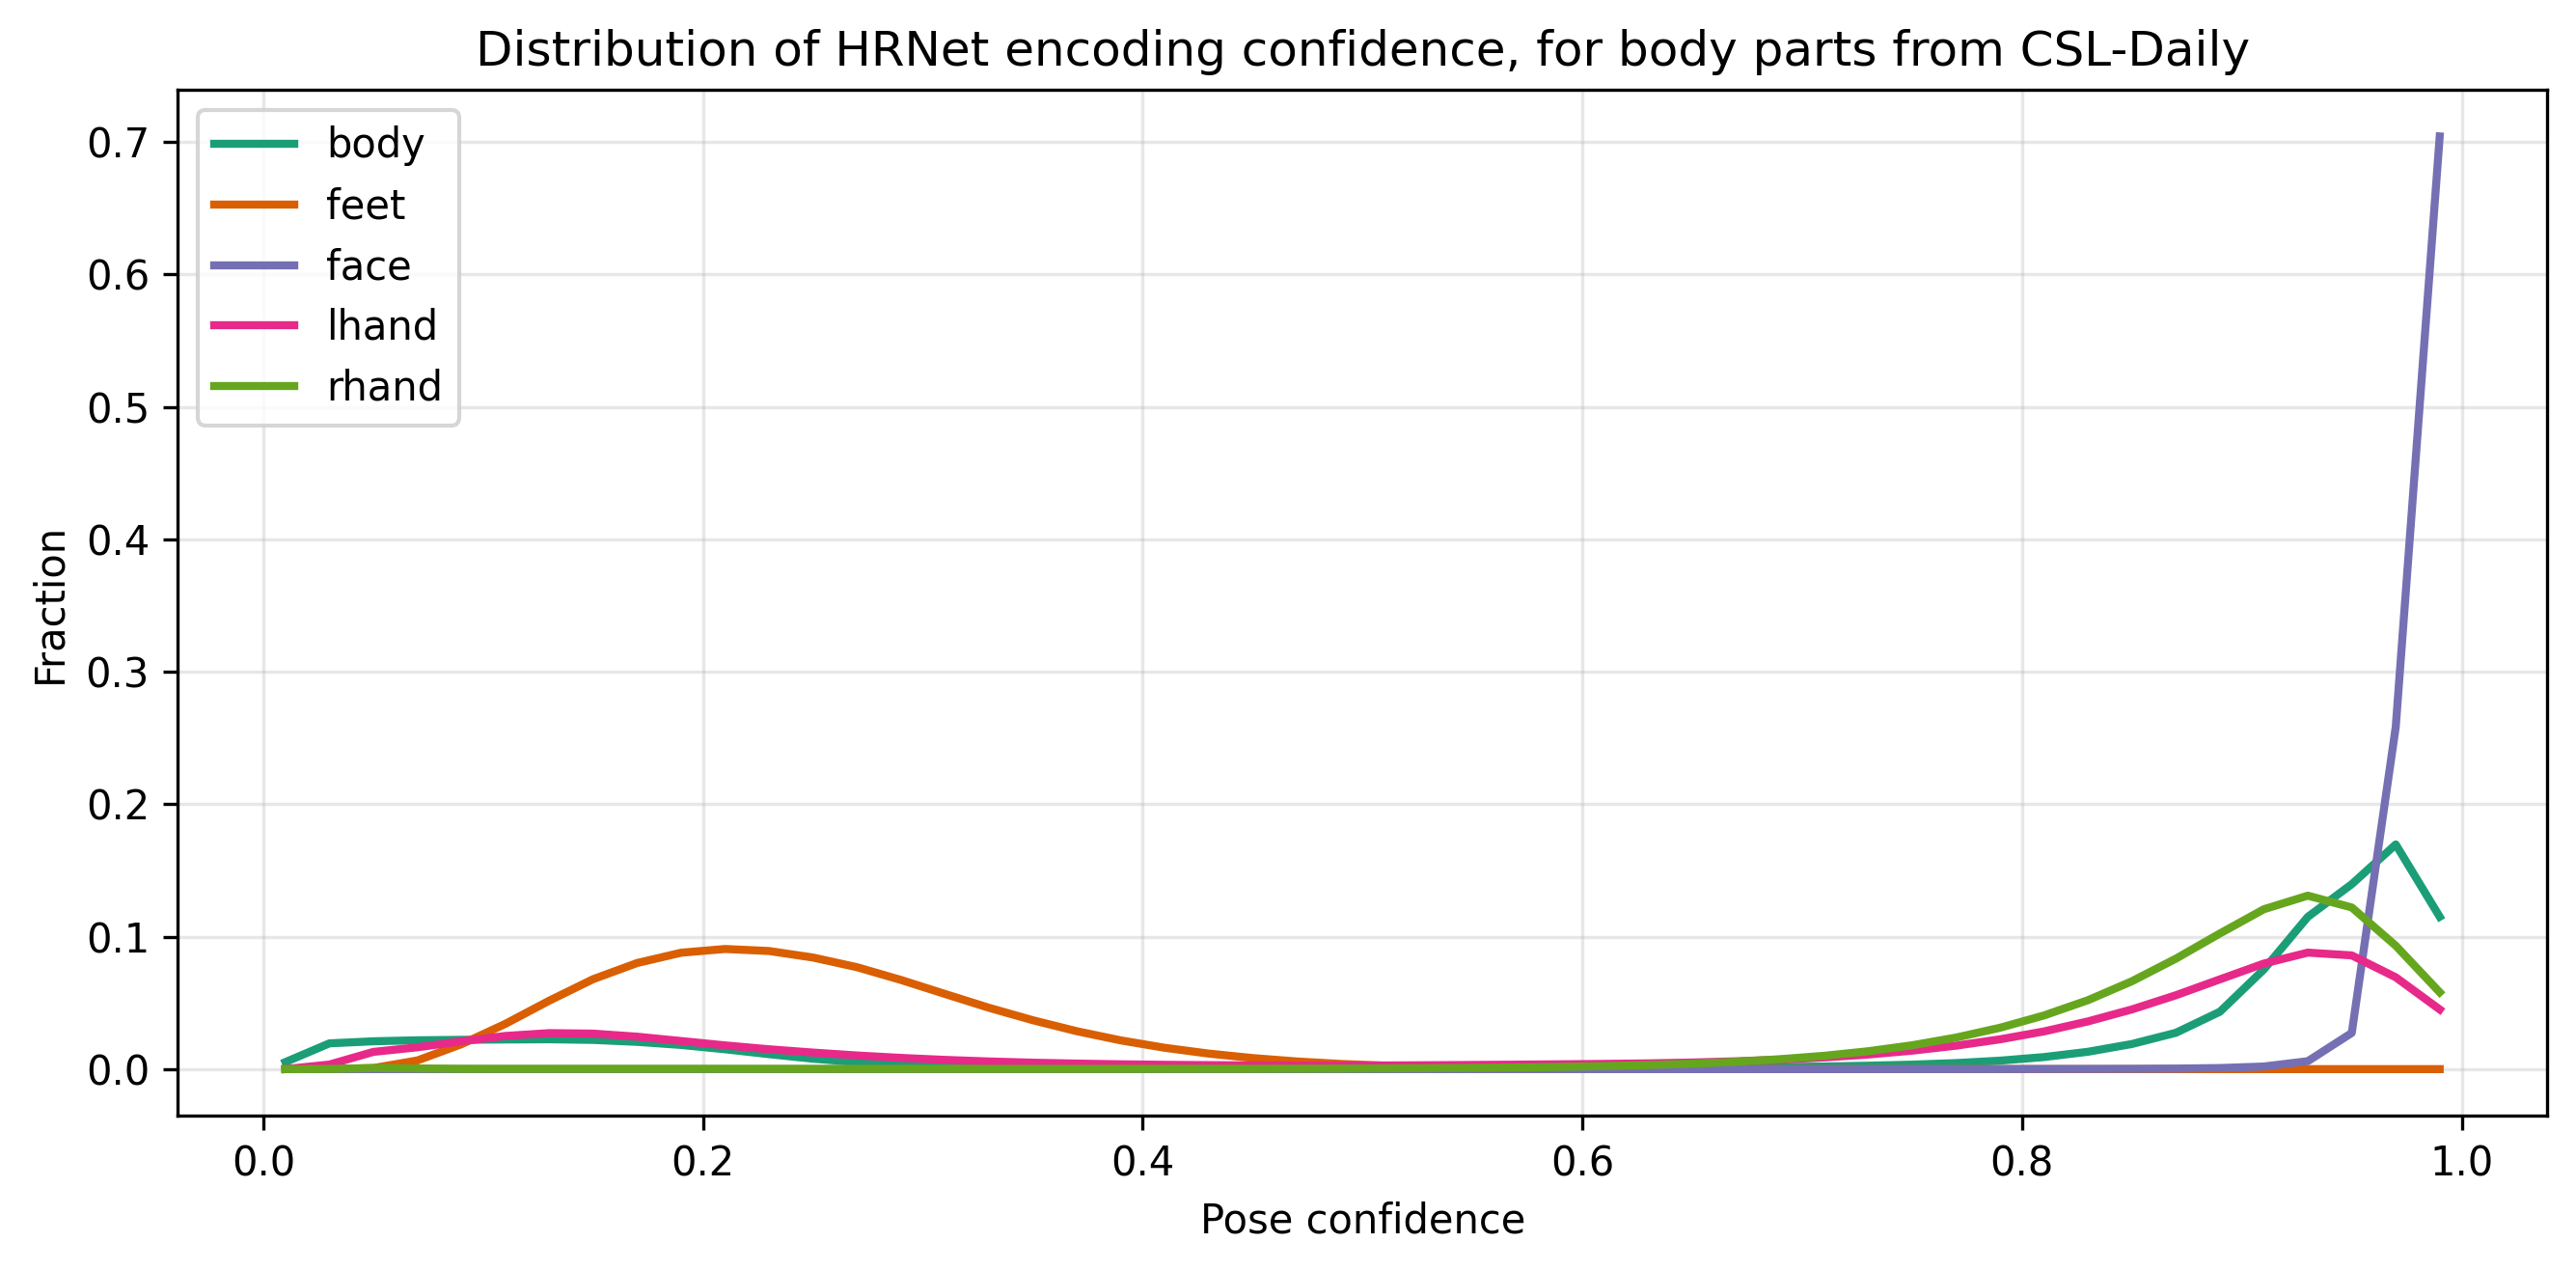
\includegraphics[width=0.92\textwidth]{HRNet_confidence.png}
  \centering
  \caption{Distribution of HRNet encoding confidence, for body parts from CSL-Daily}
  \label{fig:HRNet_confidence}
\end{figure}

\subsection{Benefits of Pre-Training}
Keypoint SLR model accuracy may be limited by the noise embedded in the datasets captured by pose estimators. Denoising Autoencoders allow reconstruction of a clean signal from corrupted noisy inputs, projecting back to the data manifold and increasing the model’s robustness to input perturbations \cite{vincent_extracting_2008}. This is only possible if the model can be trained to understand the spatial and temporal correlations of the keypoints when sign language is being performed. This may be achieved by instructing the model to recreate joints from masked inputs, training the encoder to understand the plausible movements of the keypoints by inferring them from the surrounding context both spatially and temporally. The redundant representations required for rebuilding the keypoints force the model to become more robust to corruptions \cite{vincent_extracting_2008}. The small scale of the datasets which are SLR labelled means that a larger unlabelled dataset is required to learn the data manifold. This requires pre-training with self-supervised learning before the fine tuning. 
The real-world implications of improving the robustness of models to corruptions may be larger than expected as performance is usually measured within well lit studios, whereas signing may occur in a variety of environments with restrictive lighting, viewpoints and weather effects. 
\newpage
\subsection{Key questions to answer as part of this study}
\begin{itemize}
\item Can SLR models be made more robust to inaccuracies in keypoint pose estimators by pre-training them to reconstruct the clean signal from artificially corrupted data? 
\item Does improvement in robustness translate into a marked improvement in the accuracy of the model or will the overall accuracy decrease due to a reduced ability to handle uncorrupted data? 
\item Will improvements in robustness only apply to the seen corruption types or will the robustness training improve the model for other corruptions? 
\end{itemize}
\newpage

\section{Literature Review}

\subsection{Approaches to SLR / SLT}
The transformer or attention head architecture is found across a large number of modern SLT methods. Historically there was a focus on Convolutional and Recurrent Neural Networks (CNN / RNN) within the language and translation field, but transformers appear to have surpassed these models for a variety of language related problems. Attention heads have been proven to have high performance for relatively low cost across translation models, including sign language. \cite{vaswani_attention_2023} \cite{camgoz_sign_2020} \cite{chen_two-stream_2023}. Sign2Gloss2Text models, such as MSKA, may use gloss as part of their training, by training SLR and SLT simultaneously. This avoids a bottleneck of Sign2Gloss and then Gloss2Text where residual signal from the original sign is lost when text is generated \cite{yin_better_2020} \cite{lin_gloss-free_2023}. However Sign2Gloss2Text models are limited by a lack of expertly labelled gloss datasets, whereas many more Sign2Text translation datasets are available. Gloss free models, such as Uni-Sign, rely on large scale pre-training datasets and require much more computation, often requiring Large Language Models (LLMs) as decoders \cite{li_uni-sign_2025}.

Skeleton based action recognition has become common in SLR and SLT models \cite{guan_multi-stream_2024} \cite{hu_signbert_2023}  \cite{gueuwou_shubert_2025}, but the field is still being developed with recent new tools, such as RTMPose \cite{jiang_rtmpose_2023}. However, skeleton based recognition is a mature pattern which has been used for gesture recognition for many years, with early patterns using hand crafted features and deep learning being used more recently \cite{yan_spatial_2018} \cite{shi_decoupled_2020}. HRNet \cite{wang_deep_2020} and RTMPose both perform skeleton based keypoint recognition which is the input for MSKA. Decoupled Spatial-Temporal Attention (DSTA) integrated an attention mechanism for gesture recognition after keypoint recognition and this is the backbone of MSKA's pattern encoder \cite{shi_decoupled_2020}. The body keypoints are grouped into 4 streams (left and right hands, body and face) and passed into 4 separate DSTA modules (Figure \ref{fig:estimator-streams}). The output of DSTA, when trained on sign language, will produce an embedding of a movement pattern of that body part. Pose estimators are used to generate keypoints, which are passed into DSTA. Pose estimators have known failures which may propagate through the SLR/SLT model, reducing accuracy. 


\begin{figure}[htbp]
    \centering
    \begin{subfigure}{0.48\textwidth}
        \centering
        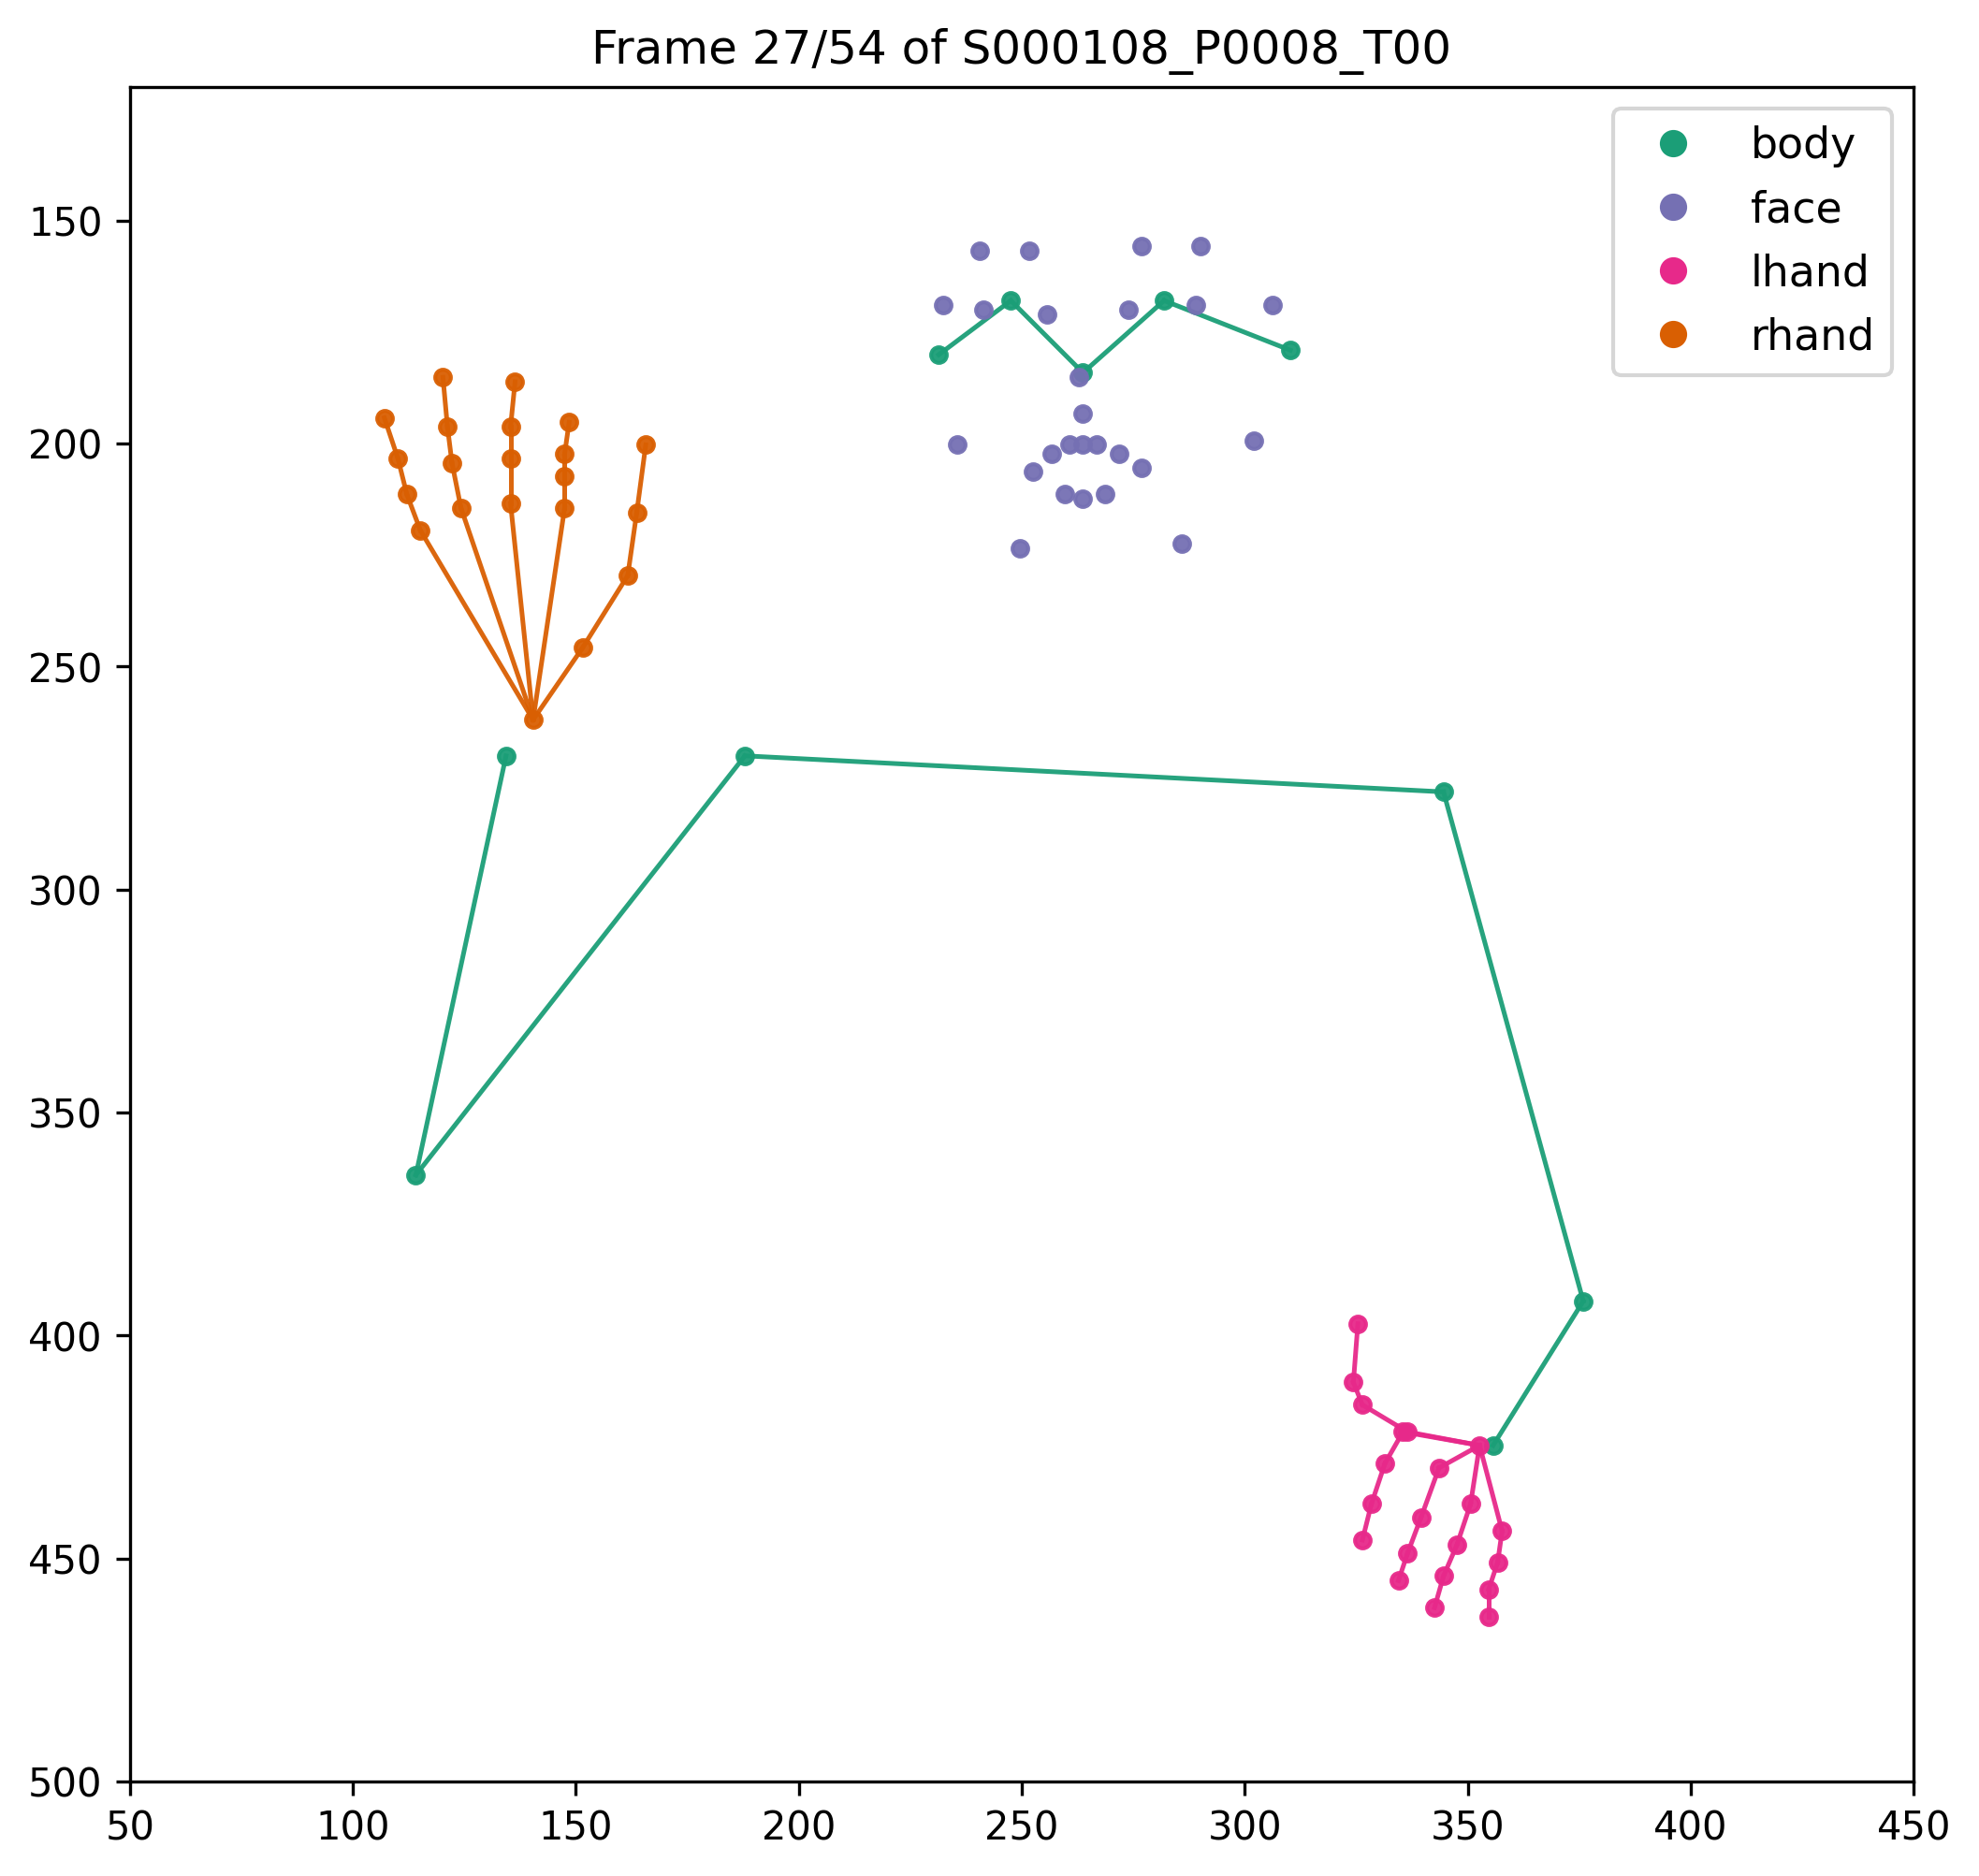
\includegraphics[width=\linewidth]{S000108_P0008_T00_body_27.png}
    \end{subfigure}
    \hfill
    \begin{subfigure}{0.48\textwidth}
        \centering
        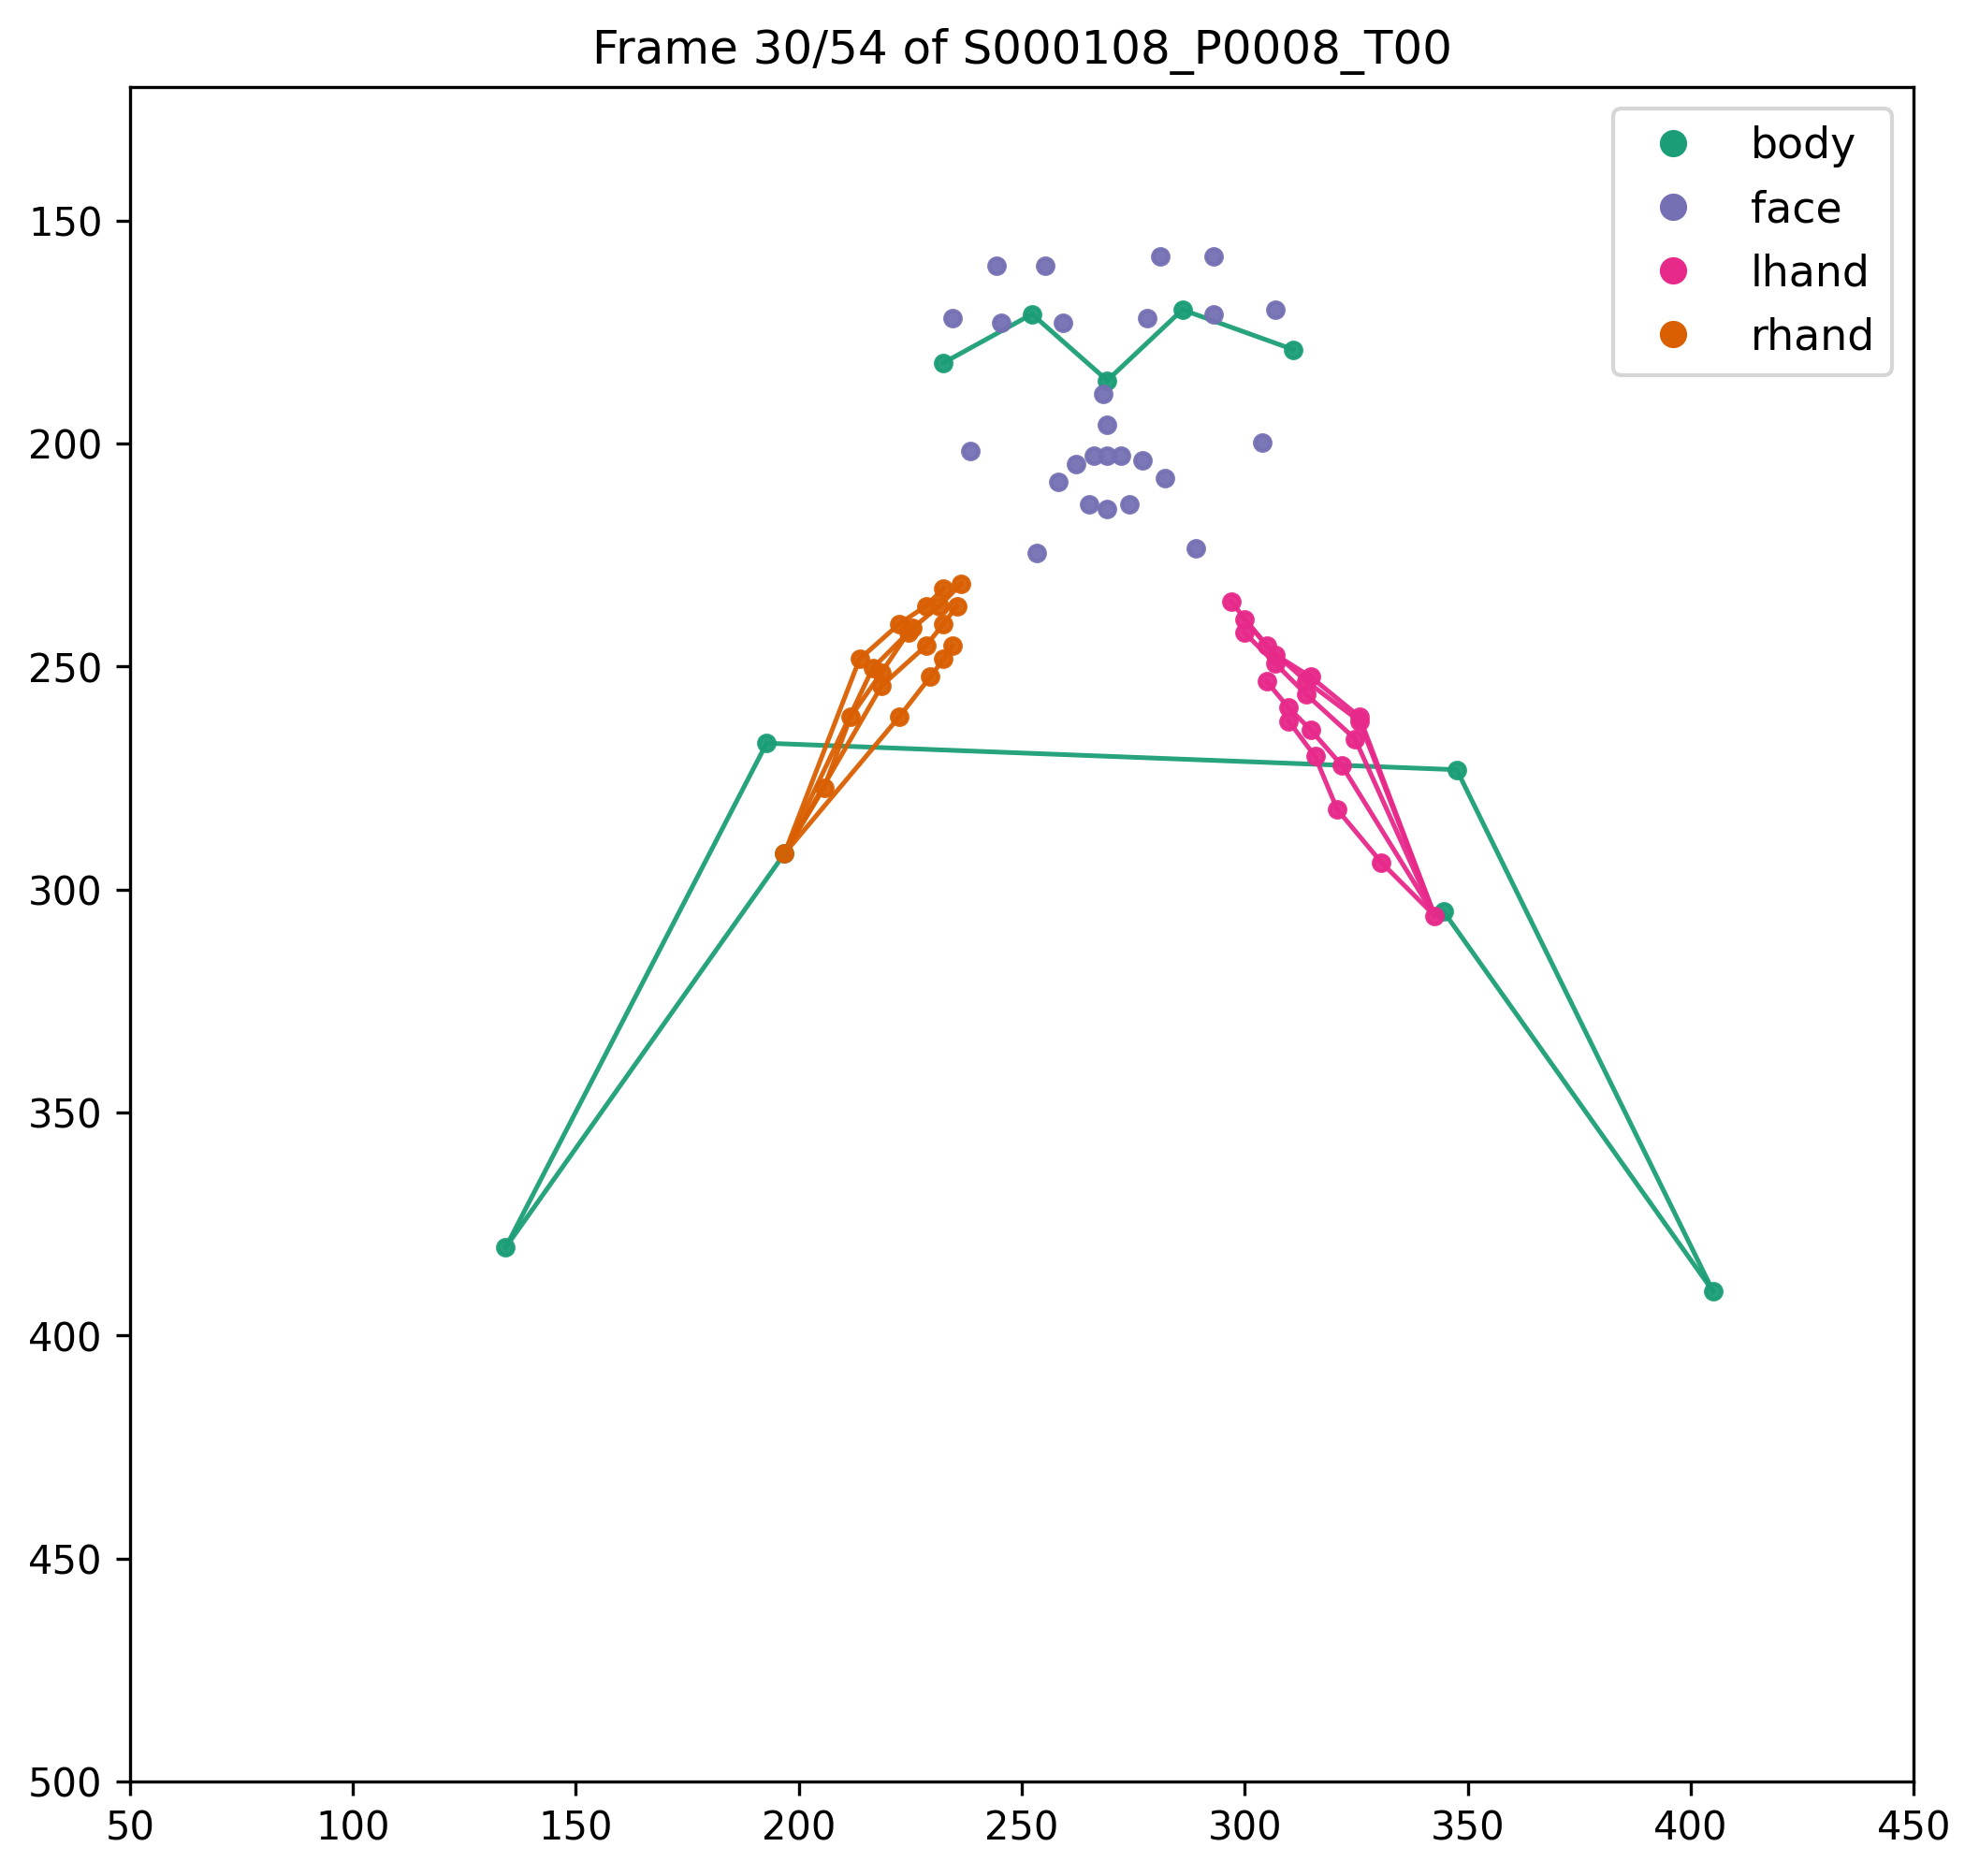
\includegraphics[width=\linewidth]{S000108_P0008_T00_body_30.png}
    \end{subfigure}
    \caption{Pose estimator keypoints and the corresponding feature streams}
    \label{fig:estimator-streams}
\end{figure}


\subsection{Pose estimator limitations}
The pose estimators RTMPose and HRNet work by first identifying humans within the image, then splitting them into face, body, hands and feet regions and then splitting those regions into keypoints. HRNet uses a heat-map based 2D gaussian distribution to find where each joint is most likely to occur. Whereas RTMPose uses coordinate classification to find the x and y coordinates of each keypoint separately. Hands are the hardest feature to recognise due to small size, frequent fast motion and occasional occlusion by other body parts. Hands may also self-occlude keypoints depending on their hand shape and orientation towards the camera.  Keypoints may be unstable and they may jitter due to noise in the original video. Additionally estimators will try to find body parts which are offscreen. For example the CSL-Daily \cite{zhou_improving_2021} dataset only contains the top half of the signer's body, but HRNet and RTMPose still attempt to locate the position of the feet .

The underlying representation of keypoints is x, y and confidence for each keypoints, with confidence representing the pose estimator's confidence that the joint was placed correctly (Figure \ref{fig:estimator-conf}). A 2d representation of objects can be restrictive, losing orientation information which may be identifiable in video data. A hand which is facing towards or away from the camera will have the same keypoint values when projected to a 2d plane. Touching of hands together or a hand to a face is common in some sign languages and this information may also be lost when keypoints are used \cite{moryossef_evaluating_2021}. Hand shape and hand movement is much more important in sign language than individual finger movement \cite{romero_embodied_2017} \cite{hu_signbert_2023}. This is mitigated in MSKA and SHuBERT \cite{gueuwou_shubert_2025}, by separating hands from the rest of the body into separate streams. The hand shape can be represented by keypoints or video and the wrist position can be used to identify the hand location \cite{gueuwou_shubert_2025}.


\begin{figure}[htbp]
    \centering
    \begin{subfigure}{0.48\textwidth}
        \centering
        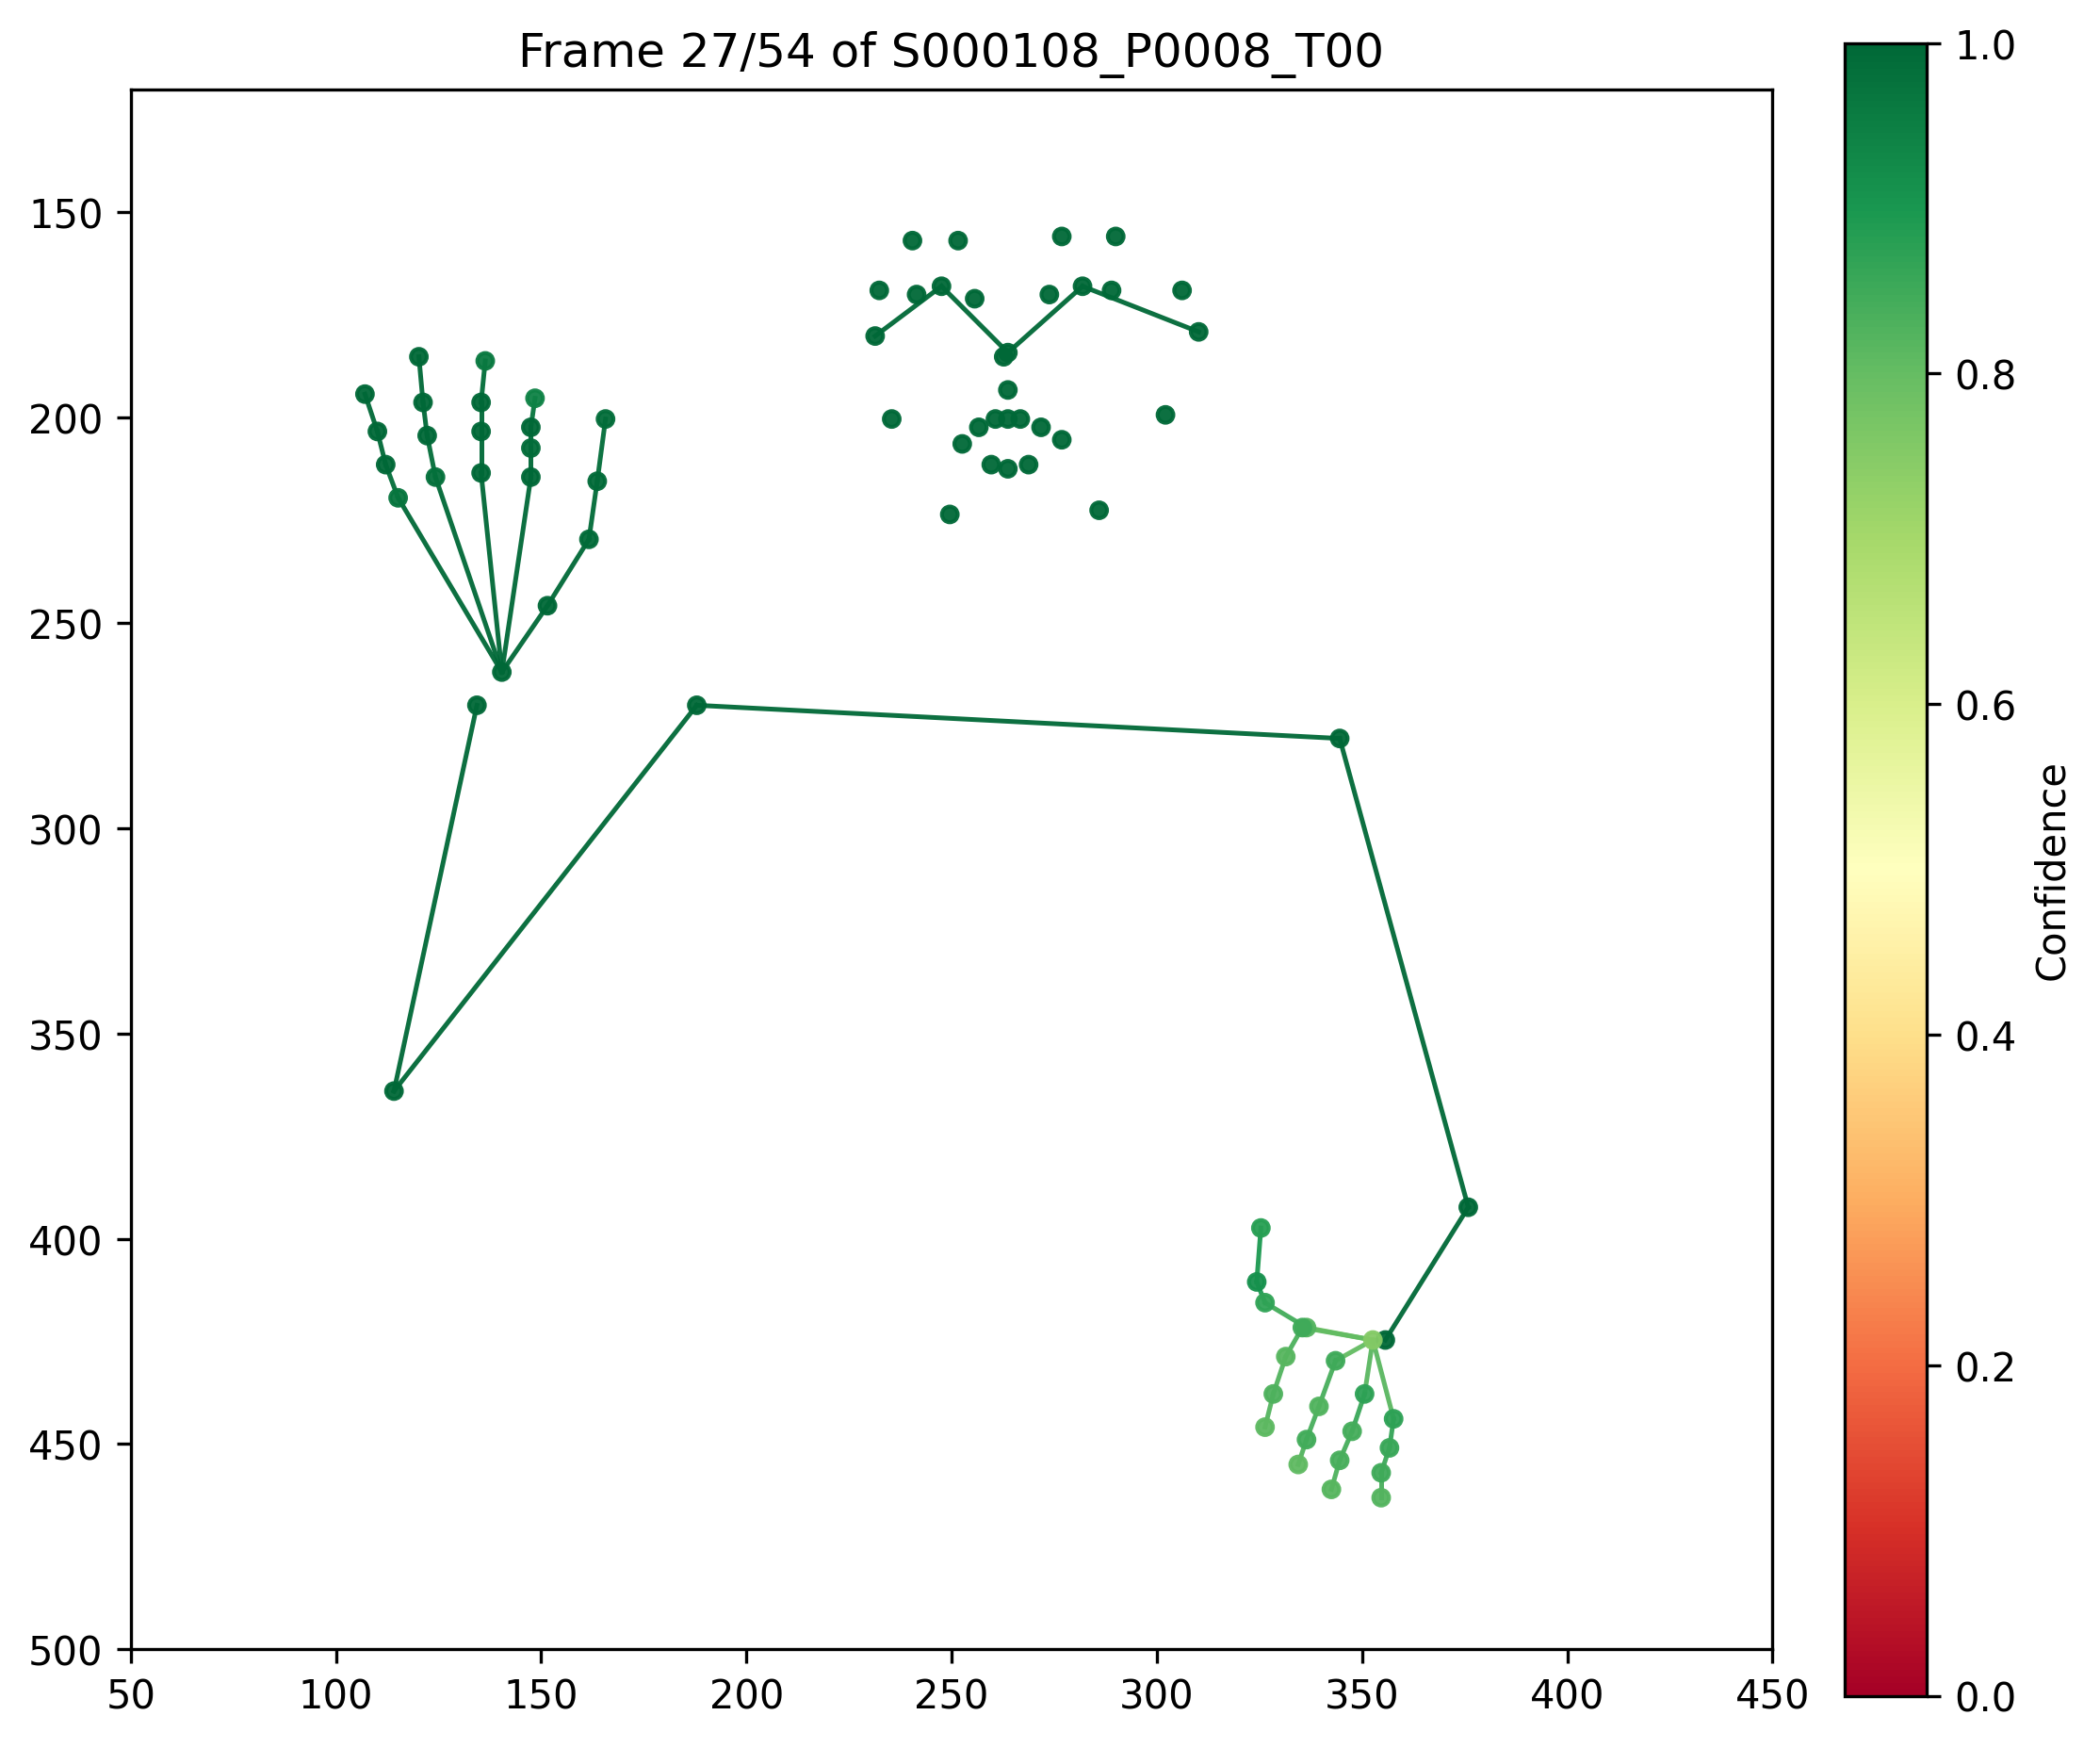
\includegraphics[width=\linewidth]{S000108_P0008_T00_conf_27.png}
    \end{subfigure}
    \hfill
    \begin{subfigure}{0.48\textwidth}
        \centering
        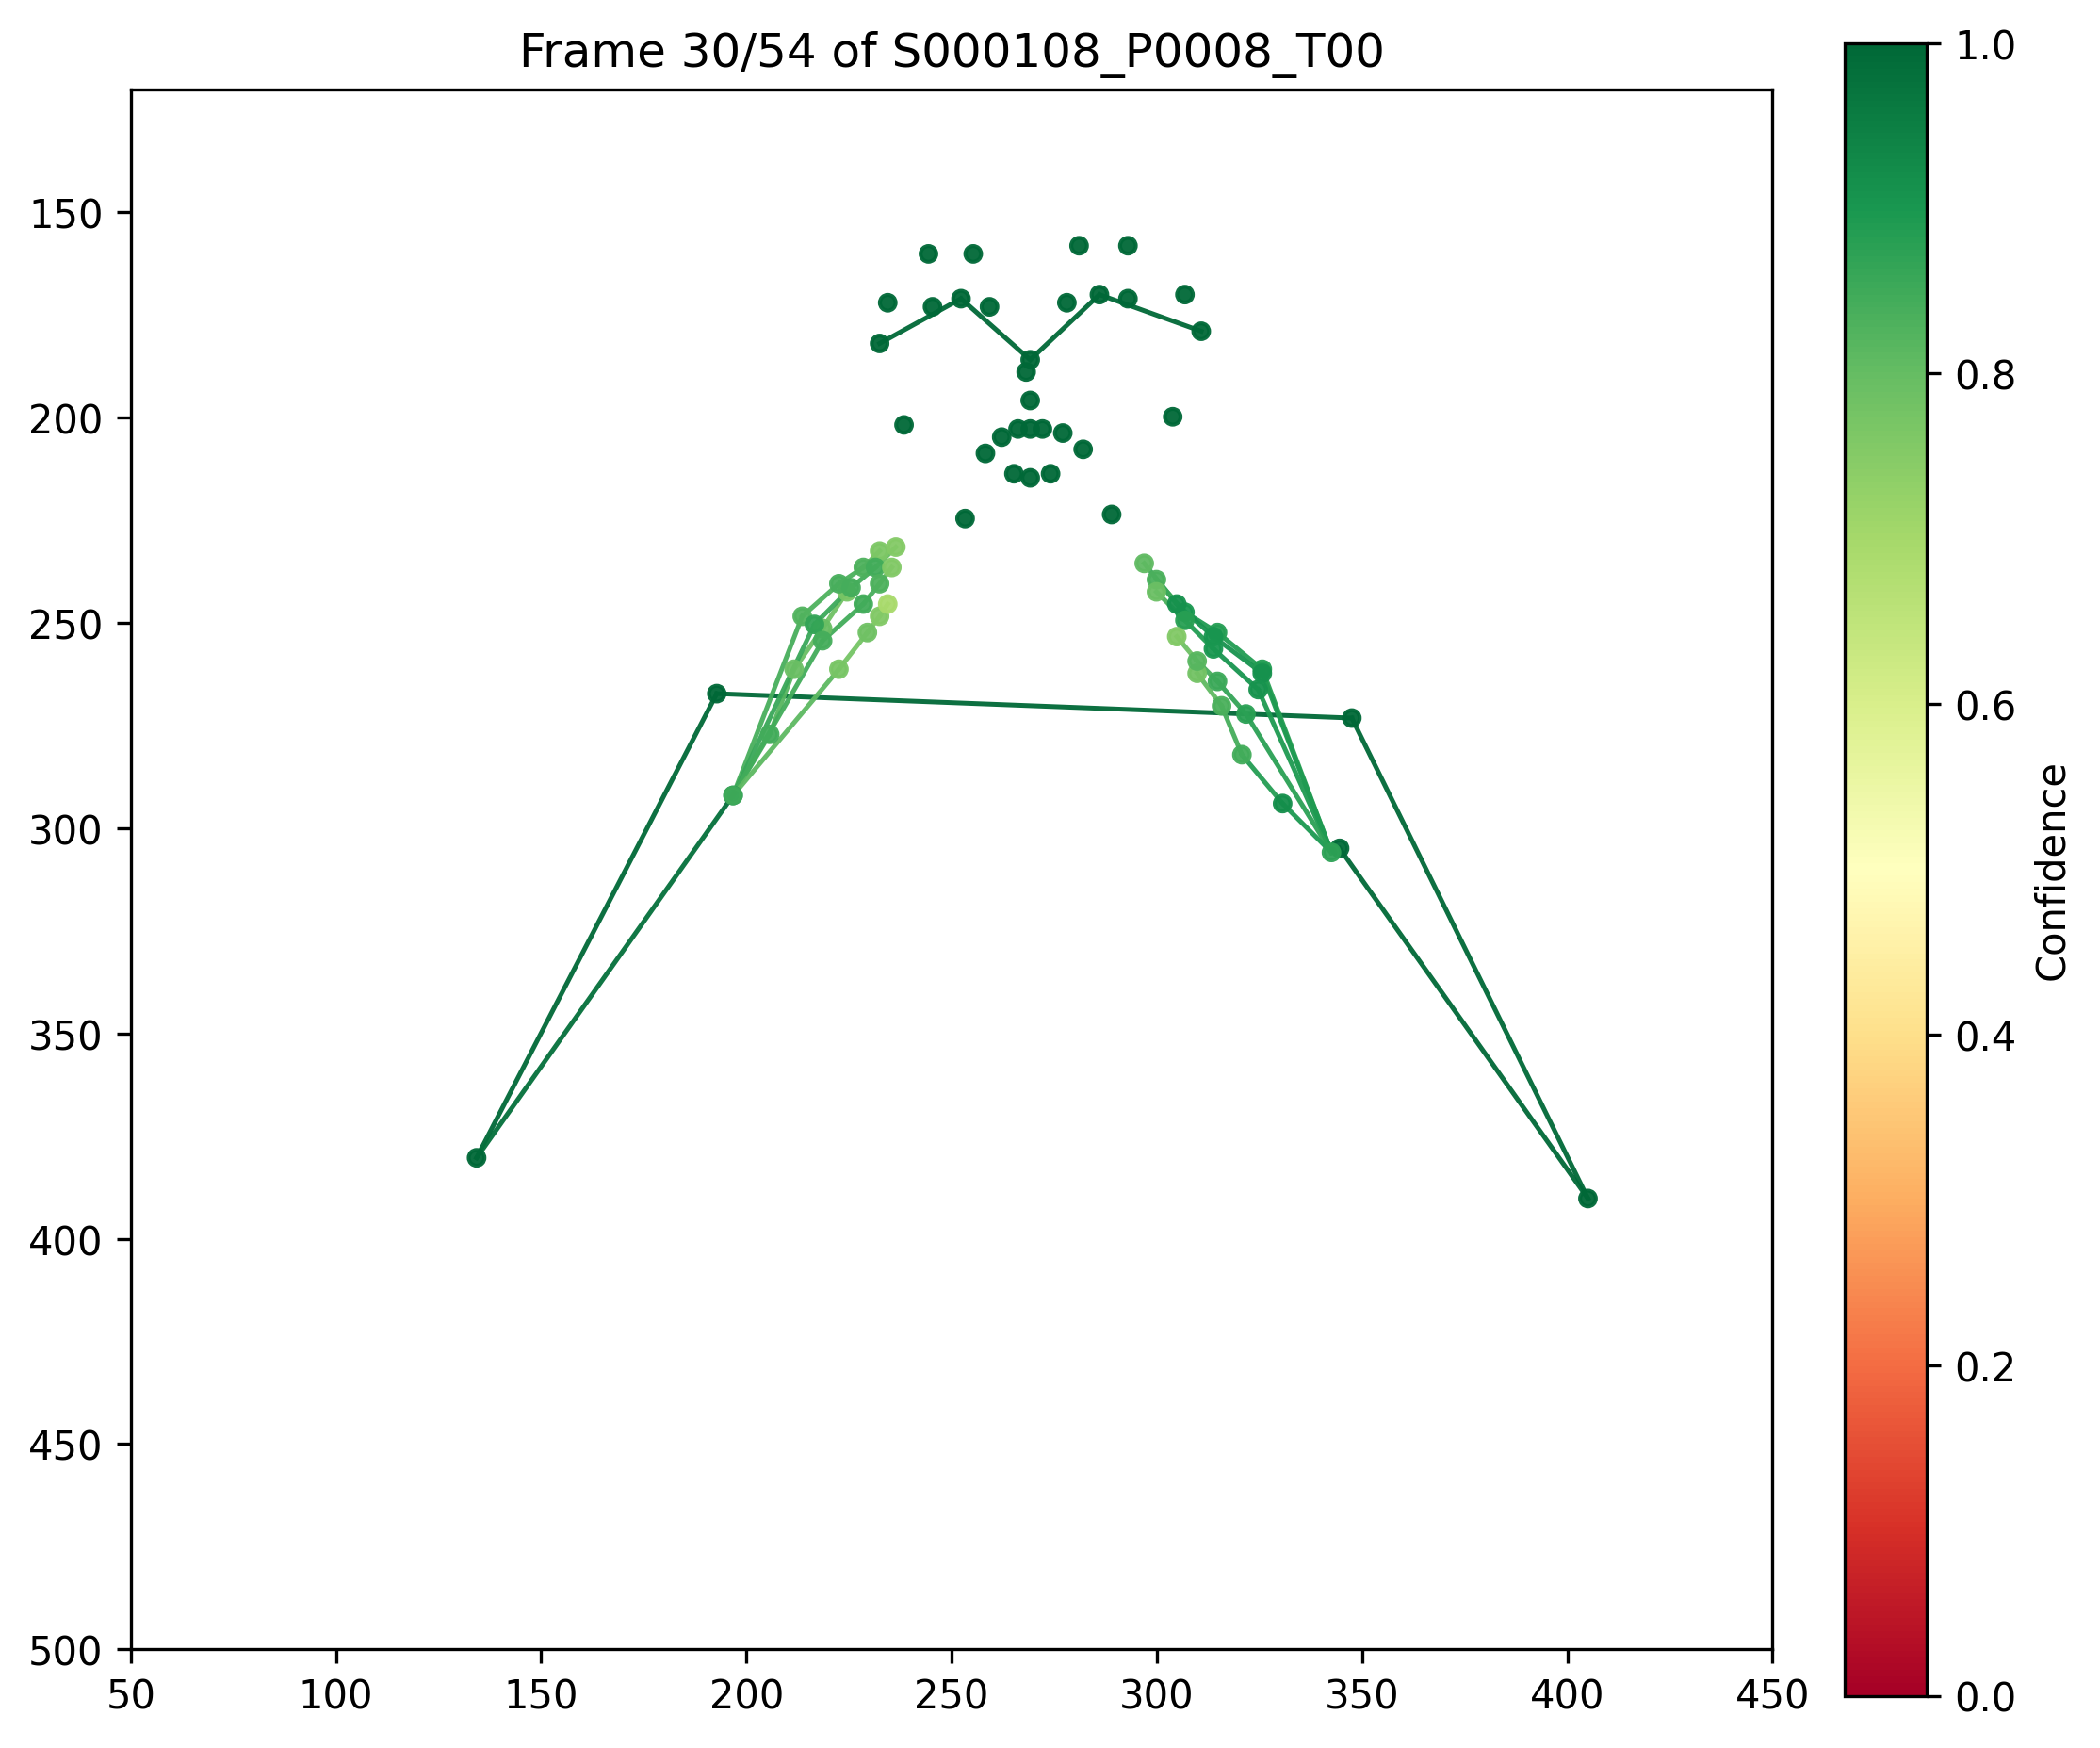
\includegraphics[width=\linewidth]{S000108_P0008_T00_conf_30.png}
    \end{subfigure}
    \caption{Pose estimator confidence levels}
    \label{fig:estimator-conf}
\end{figure}

\subsection{Self-Supervised Learning and pre-training}
Self-Supervised learning (SSL) can be used to teach language models a generic representation of a language from a large unlabelled dataset \cite{hu_signbert_2023}. SSL may reduce the amount of fine tuning required for a model, allowing a model to be pre-trained when labelled data is limited. One approach to SSL is generative learning where a model is tasked with reconstructing a signal based upon a partial signal or corrupted version of the signal \cite{liu_self-supervised_2021} \cite{vincent_extracting_2008}. A second approach is contrastive or discriminative learning, where a model is trained to identify the differences between groups within a dataset. BERT uses a generative masking based approach to SSL, training language models to better understand relationships between words \cite{devlin_bert_2019}. The BERT approach tasks the model with predicting the masked words from the surrounding context. However this relies upon discrete tokenised data, whereas sign language is continuous in nature with varying length and numbers of signs within the clips. HuBERT \cite{hsu_hubert_2021} uses a contrastive approach to SSL, assigning audio clips into clusters and then training a model to distinguish between these groups. This allows the model to be pre-trained to recognise patterns and features in continuous data. 

SHuBERT is built upon HuBERT's approach to pre-training models on continuous video features \cite{hsu_hubert_2021}. Applying this technique to Sign Language, SHuBERT pre-trains its model to assign cluster labels to sign language videos. Each video was split into multiple streams, two for the hands and one for the face and a final stream was a keypoint stream of the body. Multiple streams have been shown to be more efficient than single stream models and SHuBERT shows that they can be pre-trained, with high accuracy with field leading performance after fine tuning. SHuBERT assigns clustering once to all videos and then pre-trains the model by tasking it to assign the clusters to the video. HuBERT performs SSL iteratively, assigning clusters at each training step \cite{hsu_hubert_2021}. SHuBERT's approach may reduce training time but may also bake bias into the pre-training if the initial clustering is weak. SHuBERT's clustering is also performed against individual frames. This may lose the temporal features of the input at this training step, but this may be recovered later in the model. Temporal features have been shown to be useful when deciphering signs \cite{hu_corrnet_2024} \cite{shi_decoupled_2020}.

SignBERT performs masked generative SSL, tasking the model to reconstruct a "Model-aware hand prior" (MANO  \cite{romero_embodied_2017}) from a masked input \cite{hu_signbert_2023}. The MANO ensures that predicted hand positions align with a statistical model for the human skeleton . The model is pre-trained on many datasets across multiple languages before being fine tuned on the benchmark datasets. SignBERT can be trained separately on keypoints or video and performs well on both of these, outperforming MSKA on SLR when using video. Coordinates may be easily reconstructed from neighbouring hand joints or frames and so the model may not learn to understand the underlying features and patterns of sign language. SignBERT also uses test data during pre-training which may weaken the validity of the claims made of its performance when generalising to other datasets \cite{hu_signbert_2023}.

SHuBERT finds landmarks and bounding boxes of the hands and face, before extracting the hands and face features from those bounding boxes, which is a computationally heavy approach. SignBERT uses MMPose \cite{mmpose2020} for pose estimation, created by the same organisation as RTMPose (OpenMMLab \footnote{https://github.com/open-mmlab}). These extractors are not designed for sign language and keypoint pose estimators have known weaknesses when capturing hand shape and facial expressions \cite{gueuwou_shubert_2025} \cite{moryossef_evaluating_2021}. A clear weakness of the SignBERT model is only using the signal of hands and is not including the face or body which are known to carry signing signals \cite{hu_signbert_2023}. The ablation studies of the keypoint model MSKA show a clear improvement in SLR performance on the dataset PhoenixT when the face is included. Facial expressions, gaze and body positioning can carry meaning in sign language, but varies between languages \cite{kim_signbleu_2024} \cite{el-alfy_comprehensive_2022}.

Uni-sign is a high performing Sign2Text model which is pre-trained on the very large dataset of CSL-News \cite{li_uni-sign_2025}. Uni-Sign uses both keypoints and video as input for the model and translates directly to text during pre-training. Uni-Sign argues that pre-training sign language models by reconstructing masked inputs does not allow the model to learn textual knowledge. This suggests that these models only learn surface level visual features and this produces a gap which hinders downstream tasks such as SLT \cite{li_uni-sign_2025} \cite{gueuwou_shubert_2025}. Uni-Sign uses a large corpus of video and text with an LLM decoder which are outside of the budget of this project. (By aligning this project to the narrow focus of improving the robustness of the models to corruptions, the project can be made relevant in the SLT and SLR field without the same budget requirements.) 

Denoising Autoencoders are trained to remove noise from the input signal, projecting the input back to the data manifold \cite{vincent_extracting_2008}. The encoder is trained on a deliberately corrupted input which forces the encoder to learn the underlying patterns of the data manifold. This is one of the underlying principles behind pre-training models on masked inputs and it is the reason the robustness of the models should increase when they are exposed to corrupted data  \cite{vincent_extracting_2008}. The encoders require large quantities of data to be able to generalise, allowing the clean signal to be identified. The robustness gained by the model may be limited to corruptions which relate to the corruption that was originally trained upon. 

A linear probe is a single linear layer model which can be attached at intermediate layers of a more complex model. The probe can be trained independently to that network to better understand the features and dynamics of the layers of the larger model \cite{alain_understanding_2018}. The linear probe can be used as a fast and cheaper alternative to a full fine tune and could be used to help to identify whether the model is recognising signs. During training of the probe all layers of the larger model are frozen, allowing the probe to diagnose whether the current representation within the layers is linearly decodable to a meaningful result. This provides a tool which can be quickly and cheaply trained, allowing identification of the pre-trained model understanding of SLR. This allows us to analyse multiple pre-train variants cheaply before committing to a more expensive fine-tune. What is linearly decodable may not represent what is meaningful to the downstream part of the model as non linear functions may be required to understand the representation. Multi layer probes can be used to identify richer features within the encoder's representation, but a probe which is too large may have the capacity to learn features which are not included in the encoder's representation \cite{hewitt_designing_2019}. Therefore an appropriate probe size must be selected to ensure the probe is faithfully representing the model's understanding.

\subsection{Masking strategies}
Masking strategies can be used to train a model to meet a target based upon a partial input, the target may be the masked part of the input or relate to the target of the fine tuned model. This may allow a model to understand rules of language construction, relationships between parts of a language and make a model more robust to noise in the inputs \cite{hsu_hubert_2021} \cite{baevski_wav2vec_2020} \cite{vincent_extracting_2008}. Although they have different targets and loss functions, both SignBERT and SHuBERT attempt to pre-train the model by using a variety of similar masking techniques. SignBERT uses a naive masking technique with a limited number of masked frames. If the masking is only performed for a singular frame, joints may be too easily interpolated from neighbouring frames and this may limit the learnings of the model. A model which does not learn the data manifold will be unable to project the noisy input back to a clean signal, reducing the robustness of the model to noise. There is little ablation study to identify which techniques are most effective, however they do recognise using spatial disturbances or jitter to simulate noise in the signal. SignBERT+ is a followup to SignBERT and uses a more carefully designed masking technique mimicking issues caused by pose estimator failure. The masking techniques used by SignBERT+ include, masking all joints of a token for a limited temporal period and masking a subset of joints within a token; where a "token" appears to be a hand pose for a single frame. SHuBERT ran ablation studies on similar techniques and found the technique which improved accuracy most for SHuBERT was when masking a random channel for a small number of frames.  For keypoint SLR / SLT, the greatest performance increase and most appropriate improvements in robustness should be seen by aligning the masking techniques with corruptions identified as pose estimator failure modes. These corruptions were identified as feature occlusion and localised noise \cite{moryossef_evaluating_2021} \cite{hu_signbert_2023} \cite{jiang_rtmpose_2023}.

\subsection{Evaluation Methods and Robustness}
SLR and SLT are often trained and evaluated on limited datasets which are created in well lit studios, on limited subject matter, with clean backgrounds and limited signers. Phoenix2014T which is used to benchmark translation and recognition accuracy is from a weather forecast channel and only contains 9 signers which are all found in both the training and the test set \cite{camgoz_neural_2018}. Newer datasets such as Youtube-ASL have far broader subject matters including technical subjects and have over 2500 signers \cite{uthus_youtube-asl_2023}. However it lacks the expert labelled gloss used for SLR evaluation and also includes signers in both the training and test set. These seen test signers and limited vocabulary inflate the evaluation scores. These factors have caused academics to question whether the SLT performance of models on Phoenix2014T and similar datasets are relevant to real-world SLT \cite{tanzer_reconsidering_2024} \cite{muller_considerations_2022} \cite{yazdani_critical_2025}. A recent study has found the best SLT model performance on Phoenix2014T exceeds that of expert human performance on more generalised datasets \cite{tanzer_reconsidering_2024}. This also suggests that performance on the Phoenix2014T dataset is inflated. Due to unclear sentence boundaries, sign language may be difficult to isolate into individual sentences. Video may be split into subsections based upon pausing in hand movement or a return to a resting position. Sign language used in real-world settings is continuous and interpreters must identify pauses between phrases. 


"Signing outside the studio" investigates how models can be made more robust to background noise and how this may affect the ability of a model to perform SLT, emulating non-studio signing by replacing plain backgrounds from the original Phoenix2014 dataset \cite{jang_signing_2022}. Whilst this claims to demonstrate strong robustness to background randomization, the signers match their studio setup, being well lit, without shadow or occlusion and from a limited angle, facing directly towards the camera. Whilst the study shows techniques to identify and separate signers from background noise, the clean signal of the studio lit signer may aid in separating the signer from the background and this may not be representative of a real-world scenario.

\begin{figure}[htbp]
 \centering
  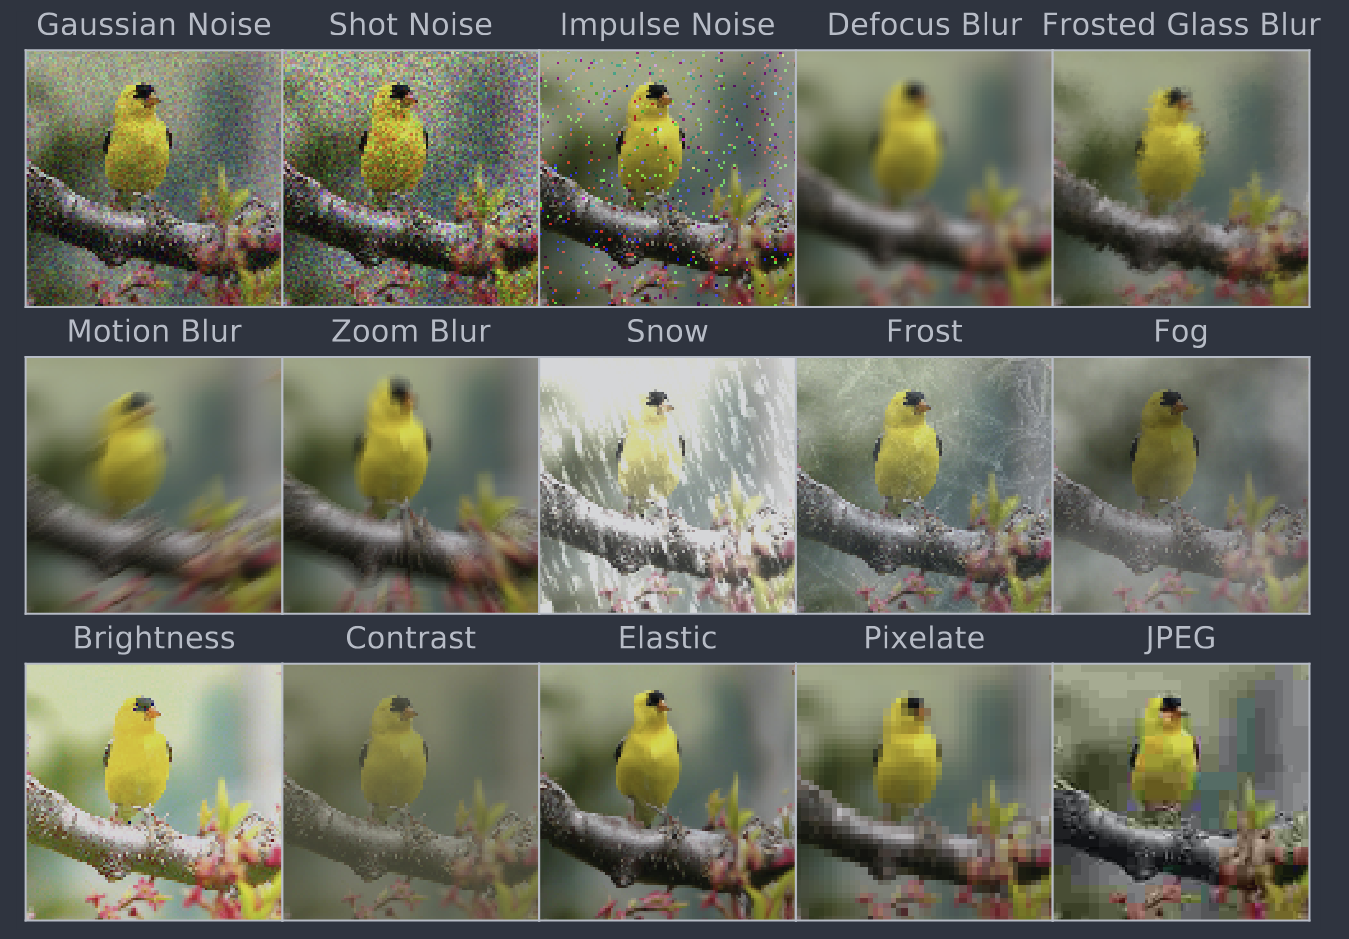
\includegraphics[width=0.9\textwidth]{imagenet-c.png}
  \caption{Still image corruptions from Imagenet-C \cite{hendrycks_benchmarking_2019}}
  \label{fig:imagenet-corruptions}
\end{figure}

Hendrycks \& Dietterich investigate 15 different types of image corruption, how they can be applied at differing severity levels and how this affects identification of images from the ImageNet dataset. \cite{hendrycks_benchmarking_2019} \cite{deng_imagenet_2009}. The corruptions are in 4 groups; noise, blur, weather and digital. Studio based sign language videos are not affected by weather, but are likely affected by gaussian noise, focus or motion blur and digital artifacts such as pixelation and compression(Figure \ref{fig:imagenet-corruptions}) . These corruption methods are appropriate for images but lack the corruptions that may occur from the temporal factors of video. Schiappa et al. builds upon image corruptions, identifying how camera rotation and shake could affect a video as well as temporal issues such as freezing and varying sampling rate \cite{schiappa_large-scale_2023}. Corruptions should be selected which can be accurately reproduced upon keypoints, with robustness analysis noting which corruptions were seen and unseen when training the model. Schiappa et al. identifies how robustness curves can be used to identify how each model performance decreases as corruption severity increases. The models are tasked with predicting targets from corrupted versions of the inputs, with the experiment repeated for multiple types of corruption and at multiple corruption severities. Model degradation relative to the existing baseline model is observed as this will show changes in the model's robustness to the tested corruption.

\newpage
\section{Method}

% TODO architecture diagram

\subsection{Data pipeline}
\subsubsection{Keypoint datasets}
A key goal of this project is to identify whether a model can be pre-trained to better understand sign language being performed in order to improve the accuracy and robustness of the model after fine tuning. It is important to find a large sign language dataset which is of high quality and can be accessed and processed within the budget of this project. MSKA SLR and SLT were benchmarked using the Phoenix and CSL-Daily datasets in the languages German Sign Language (Deutsche Gebärdensprache DGS) and Chinese Sign Language (CSL). Pre-training can be performed across multiple languages and a new benchmark could be created for MSKA SLT using alternative languages, but datasets with expertly labelled gloss for SLR benchmarking are limited \cite{vedaldi_bsl-1k_2020}. There is a high cost of encoding video to keypoints and so datasets which are already encoded are very useful for the project as they save time and budget.    

The dataset CSL-News was collated for the Uni-Sign project and based upon 1,985 hours of Chinese news television, with textual annotations extracted, but without gloss. The keypoints for this dataset have been extracted using RTMPose which is a light pose estimator framework. The MSKA paper uses the pose estimator HRNet model to extract keypoints from the original video dataset. The CSL-News dataset is well suited for our method, as the large size of the dataset should be sufficient to allow the model to be trained to generalise how hands move during sign language. The language of the dataset matches the CSL-Daily benchmark and keypoint encoding of the dataset is well suited to this project.

RTMPose has been shown to have equivalent performance to the pose estimator HRNet and is commonly used, due to it requiring less processing power than HRNet. To ensure consistency across the experiment, keypoints extraction for CSL-Daily needs to be performed with RTMPose; these keypoints are also provided by Uni-Sign. MSKA uses 79 of the 133 COCO-WholeBody keypoints created by HRNet and RTMPose. Alignment of the order of the keypoints by each pose estimator must be ensured so that the keypoints are correctly split when passed into the 4 streams that constitute the MSKA architecture. 

\subsubsection{CSL-News}
The CSL-Daily dataset is based upon high resolution, studio captured images with a resolution 1920 x 1080 whereas the CSL-News contains images which are in the order of 220 x 220. This is due to the video being captured from a small box containing the signer in a cropped corner of the TV broadcast. The original resolution of the video can affect the performance of the pose estimator and the confidence of the keypoints produced, this can be seen in the Figure \ref{fig:CSL_confidence} with CSL-News showing a reduced confidence in the hands. However the model will automatically handle changes in resolution as keypoints passed into the model are normalised with coordinate scaling. The coordinates are scaled by the approximate size of the signer to ensure consistency across resolutions, signer sizes and camera distance. The coordinates of the keypoints are unclipped as the pose estimator may predict that a specific keypoint will appear outside of the video. This behaviour is expected as hands are often at rest between signed sentences and may come to reset at the edge of a frame. The video is cropped to waist height so feet are never present as sign language is performed with the upper body. Additional noise due to the lower resolution of the dataset can be accommodated by selecting clips based upon the  keypoint confidence. The CSL-Daily dataset is a studio based, high resolution dataset and may not contain the same corruptions that may be present in videos captured in less noisy settings. This may result in a limited improvement to the performance of the model on the CSL-Daily dataset when it is trained to be more robust. However the less corrupted keypoint data of CSL-Daily allows each corruption approach to be run in isolation of other potential corruptions.

\begin{figure}[htbp]
  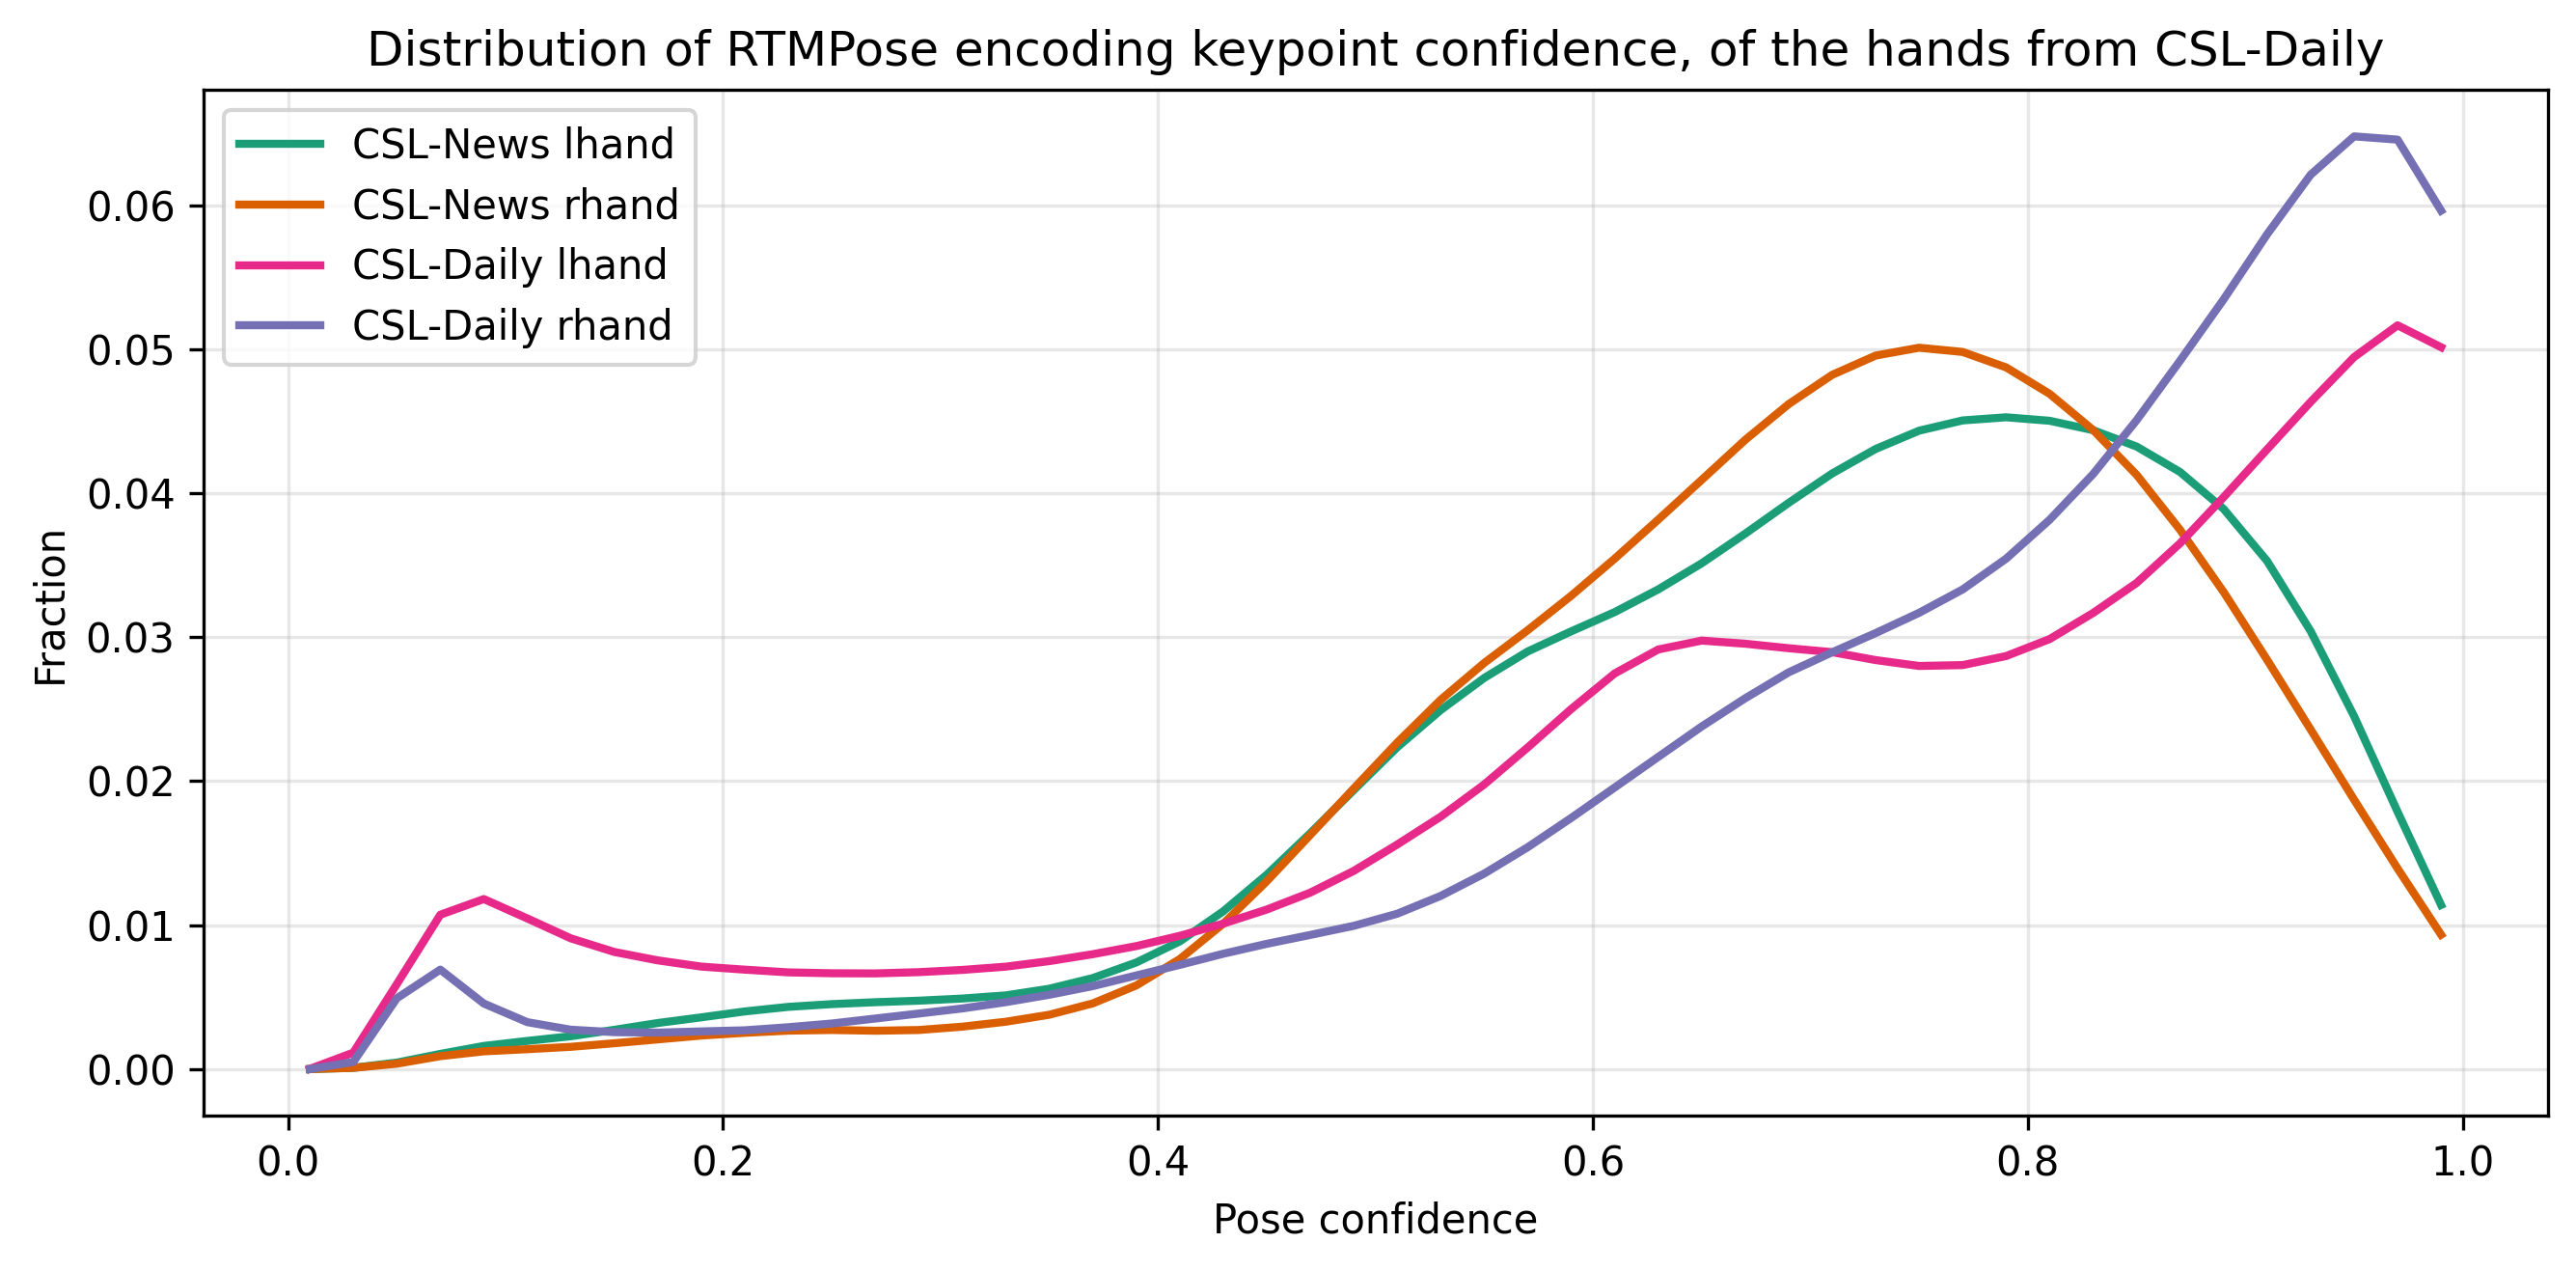
\includegraphics[width=\linewidth]{CSL_confidence}
  \caption{Distribution of RTMPose encoding keypoint confidence, of the hands from CSL-Daily}
  \label{fig:CSL_confidence}
\end{figure}

During analysis of fine tuning the baseline model, after 10 epochs of fine tuning, it was estimated that each fine tune would take approximately 80 hours on a g5.xlarge which costs around 1.1 dollars per hour. This would only allow a budget for one baseline fine tune and one experiment fine tune. To allow for more experiments and studies the frame rate of the keypoints was halved and spot instances were used, together this reduced the cost of each fine tune by around 80 percent. 

The CSL-News\_pose dataset is 256GB hosted on huggingface \footnote{\url{https://huggingface.co/datasets/ZechengLi19/CSL-News\_pose/tree/main}} across 46 archives. To process the dataset so that it could be used by the model, 10 non sequential archives of the 46 available were downloaded. These were extracted, the frame rate was reduced by half and they were shuffled into 75 shards. These were stored on S3 and could more easily be loaded onto EC2 instances for pre-training.

\subsection{Ensuring the experiment is comparable and meaningful}
After making changes to the pose estimator, by using RTMPose rather than HRNet, as well as adjusting the frame rate, the experiment must be ensured to be meaningfully comparable to the MSKA baseline. An analysis of the keypoints produced by the two pose estimators was performed. HRNet produced keypoints which were on average 0.7 of the length of RTMPose, the fractional difference in length was not consistent and varied between 0.51 and 0.93, with RTMPose longer in all examples (before the frame rate was reduced) (Table \ref{hrnnet_rtmpose}).  

To normalise keypoint positions, ensuring consistency across signers and resolution, MSKA uses shoulder width and location. The keypoints of the shoulders are identified and located, the midpoint between them is calculated and used as the origin. The keypoints are then normalised based upon the distance between the shoulder, centring on the origin. The units in Figure \ref{fig:both_wrists} and Figure \ref{fig:pose_distance} are signer shoulder-widths. Visually examining the differences in the keypoints from the two pose estimators in Figure \ref{fig:both_wrists}, the paths of the wrists appear to be following very similar non trivial paths. HRNet appears to have been clipped, with shorter movement paths than RTMPose. A Python script was used to maximise the section of the wrist paths which were most similar across both pose estimators. This clipped the ends of the paths and then resampled them to ensure a consistent frame rate, the distance between the wrists was then measured at each frame. The clipping was then applied to all keypoints. This was performed on 1000 randomly selected examples. In Figure \ref{fig:pose_distance} the distance between the two estimators for the face and body keypoints is very small for most examples with the left and right hand matching less well. This may be due to obstruction, motion blur or out of frame keypoints for these groups as the left hand is more often at rest and out of shot. The keypoints of RTMPose and HRNet were shown to align, allowing the project to continue with the use of RTMPose. The confidence in each keypoint was not accounted for in this analysis.

Word Error Rate (WER) is used to measure the accuracy of SLR when comparing the expected and predicted gloss and is calculated by comparing the Levenshtein distance of the expected vs actual result. All WER in this paper are shown as percentages with lower values indicating higher performance. A fine tune of the MSKA model was performed using the RTMPose CSL-Daily keypoint dataset at half the frame rate of the original videos. This created a baseline which could be compared against the original MSKA paper as well as experiments relating to fine tuning after pre-training. This baseline WER was 28.2 which is very close to the fine tuned HRNet full frame rate WER at 27.8. This is a significant result and shows that RTMPose at half the frame rate is meaningfully comparable to HRNet. 

\begin{figure}[htbp]
  \centering
  \begin{subfigure}[t]{0.48\textwidth}
    \centering
    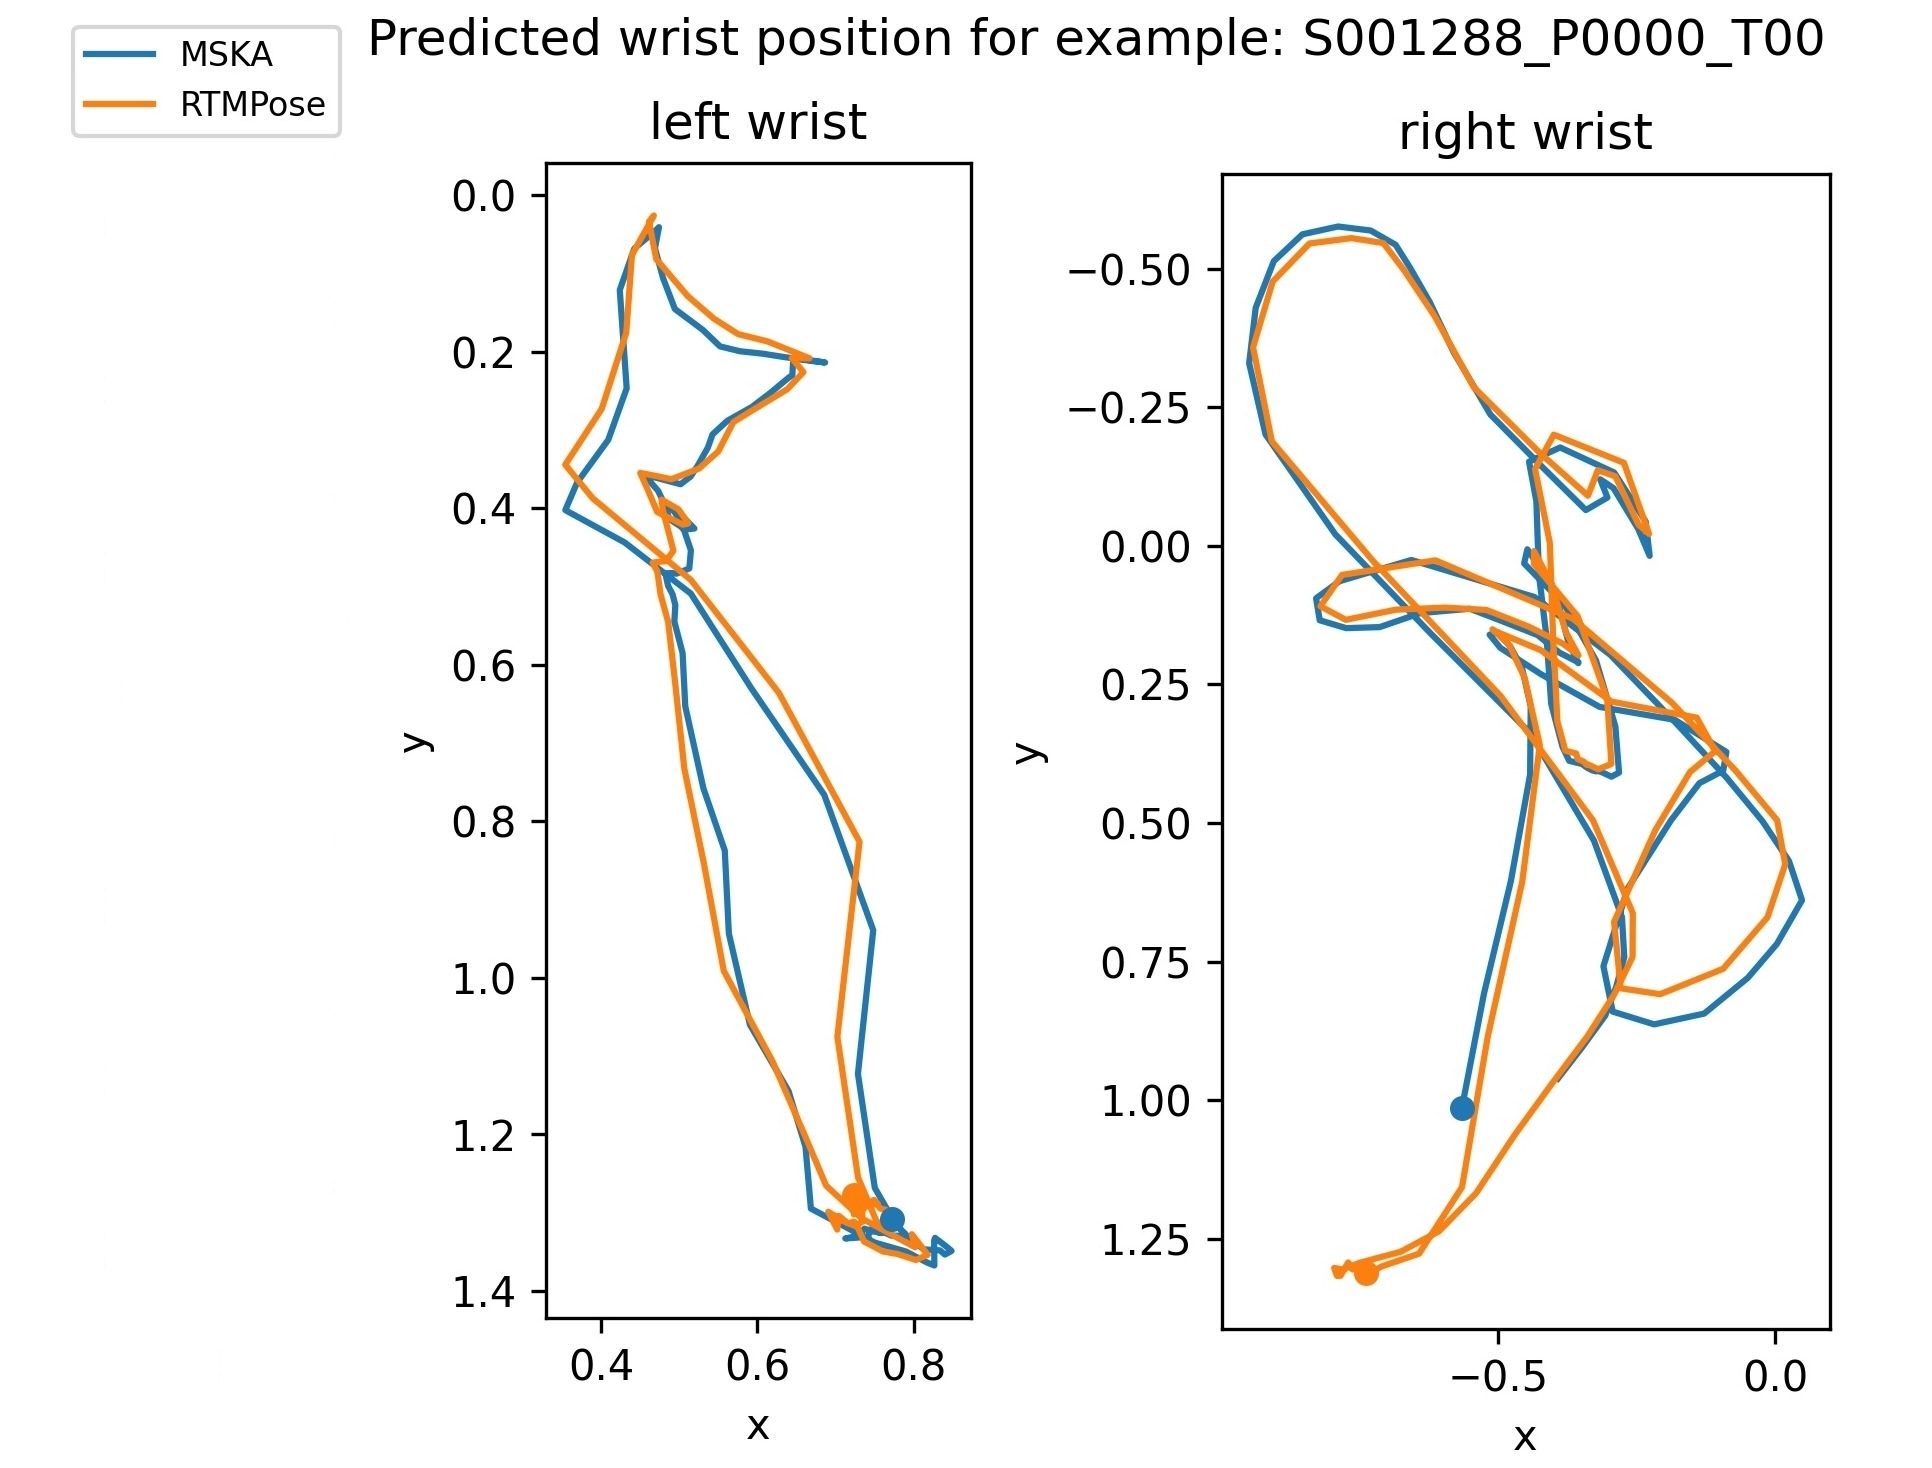
\includegraphics[width=\linewidth]{predicted_wrist_path_1288.jpg}
    \label{fig:wrist_1}
  \end{subfigure}
  \hfill
  \begin{subfigure}[t]{0.48\textwidth}
    \centering
    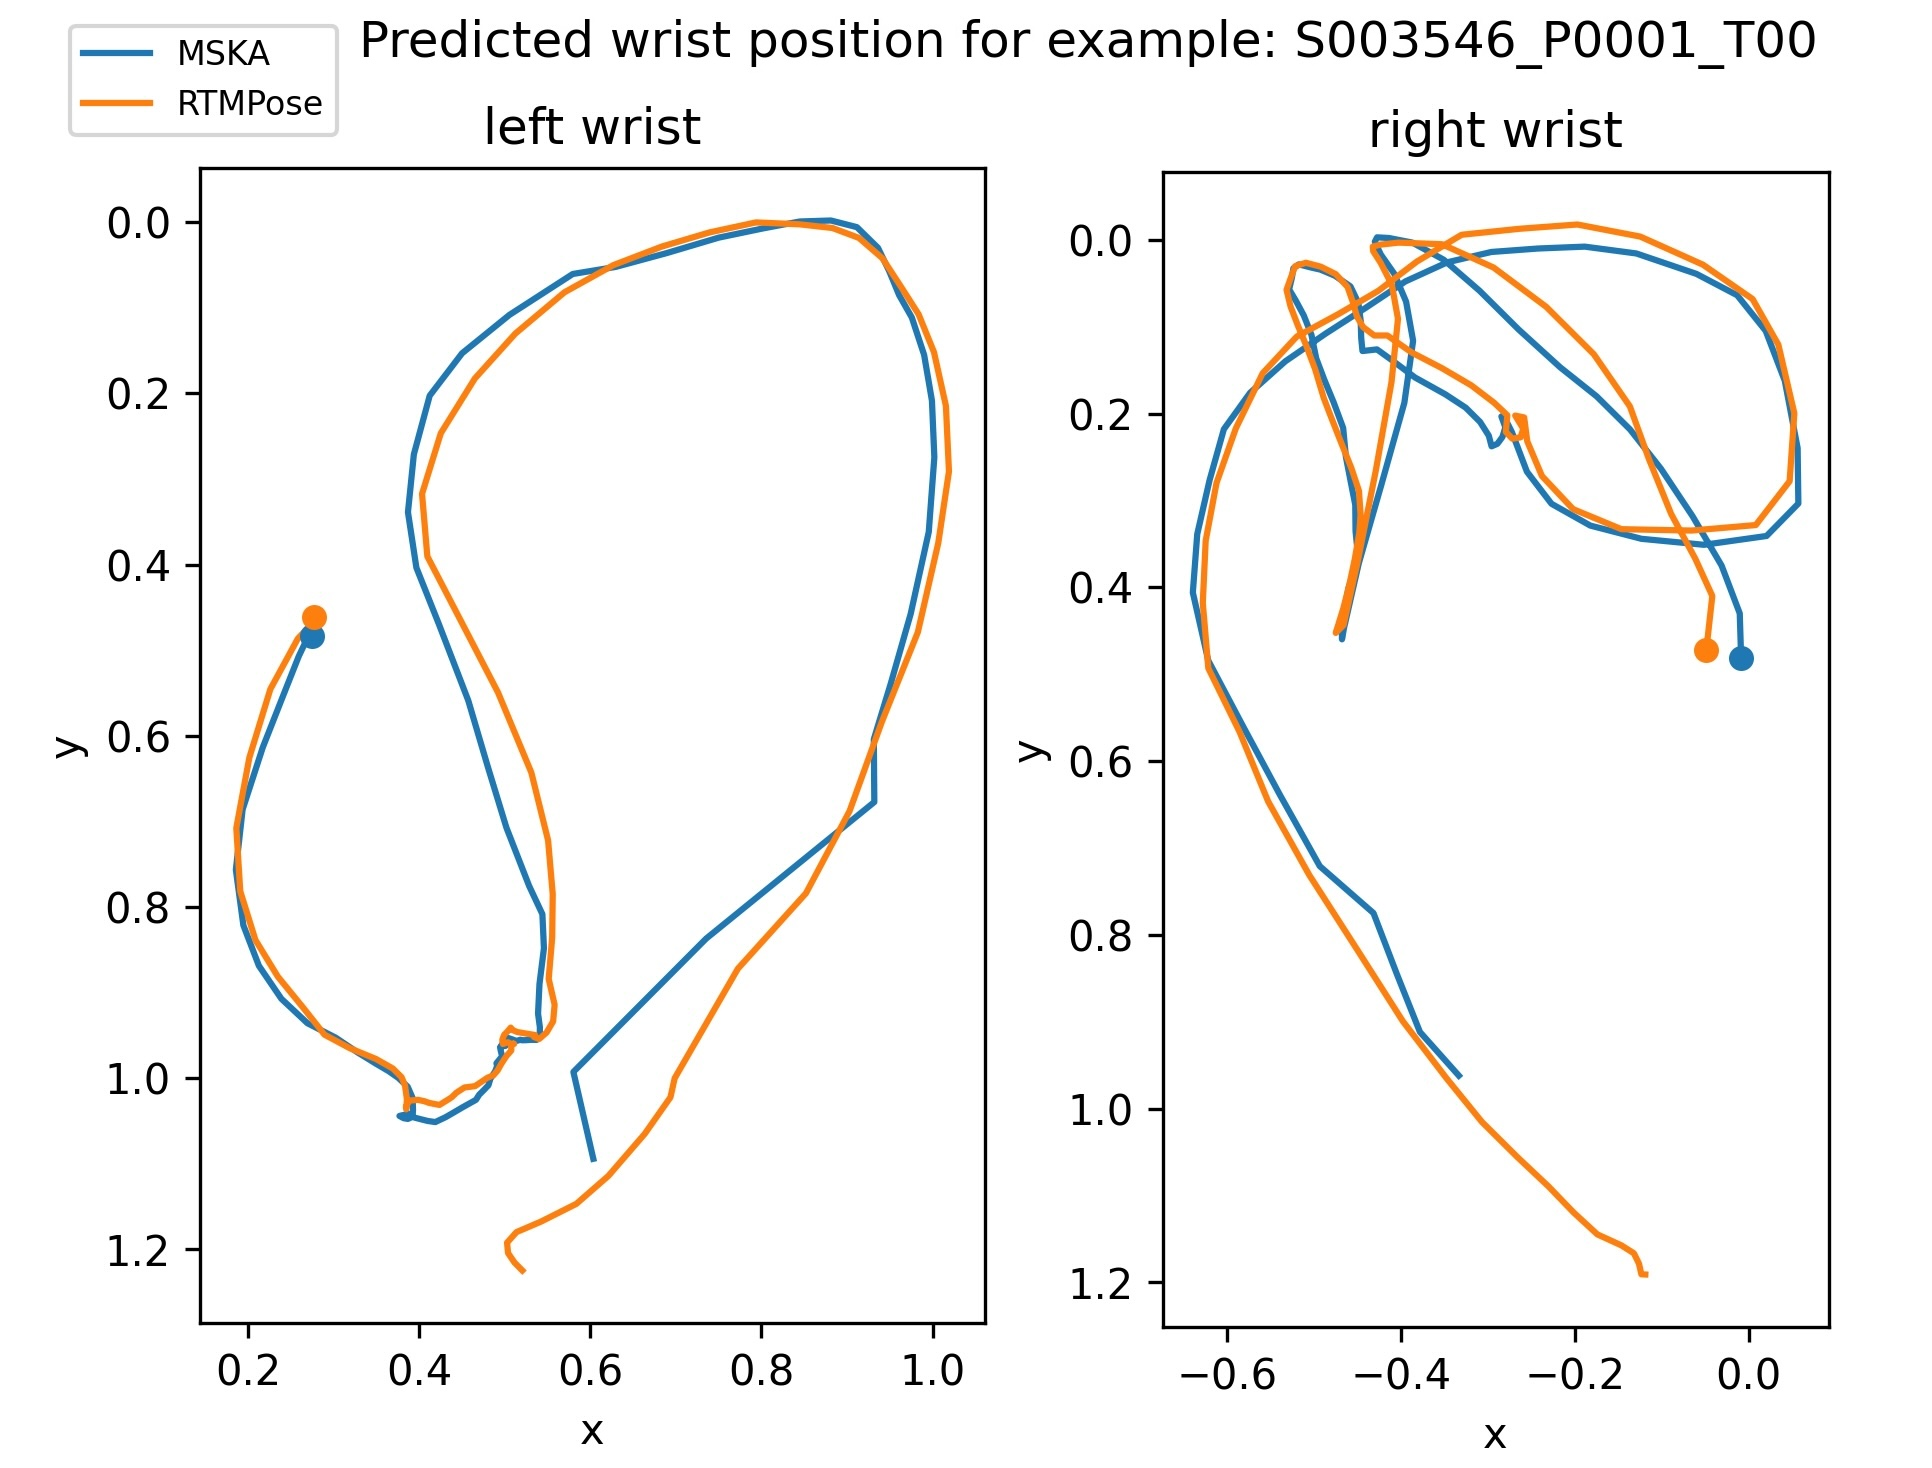
\includegraphics[width=\linewidth]{predicted_wrist_path_3546.jpg}
    \label{fig:wrist_2}
  \end{subfigure}
  \caption{Selected examples of wrist paths for HRNet and RTMPose}
  \label{fig:both_wrists}
\end{figure}

\begin{table}[htbp]
  \centering
\begin{tabular}{|c|c|c|c|c|}
    \hline
      & Mean & Min & Median & Max \\
    \hline
    HRNet Len & 137.4 & 57.0 & 119.0 & 253.0 \\
    \hline
    RTMPose Len & 189.2 & 87.0 & 190.0 & 346.0 \\
    \hline
    Fraction & 0.708 & 0.514 & 0.709 & 0.934 \\
    \hline
    Difference & 51.8 & 12.0 & 44.0 & 93.0 \\
    \hline
  \end{tabular}
  \caption{Frame length (number of frames) of HRNet and RTMPose clips}
  \label{tab:hrnnet_rtmpose}
\end{table}

\begin{figure}[htbp]
  \centering
  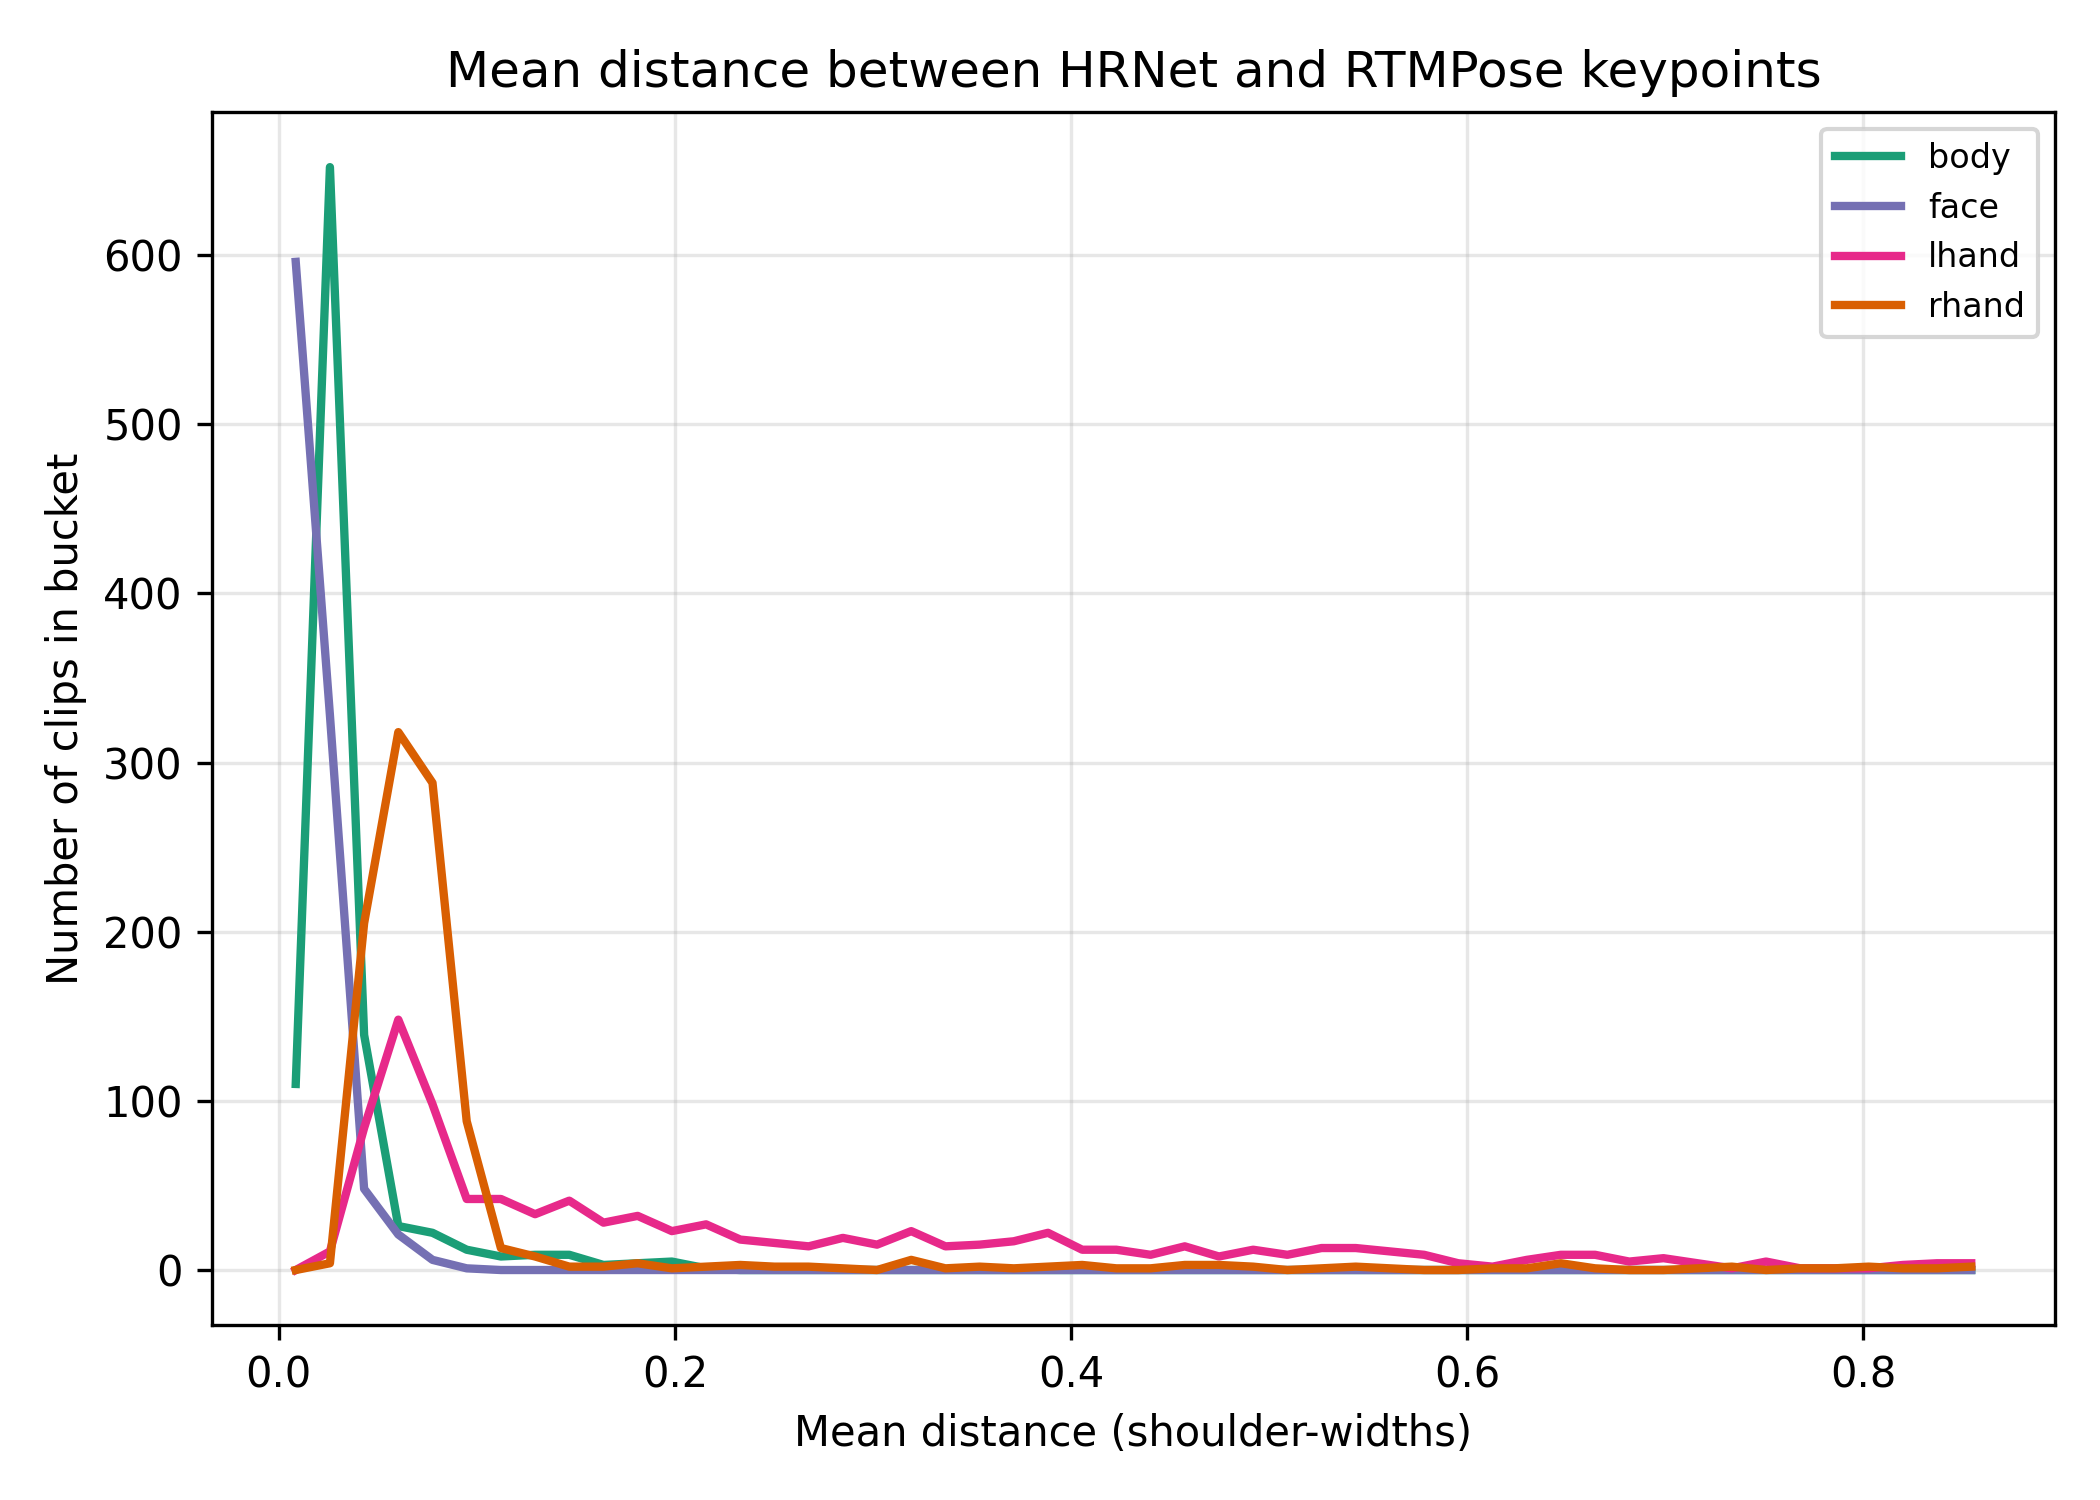
\includegraphics[width=0.9\textwidth]{pose_distance.png}
  \caption{Mean distance between HRNet and RTMPose keypoints for body parts from CSL-Daily}
  \label{fig:pose_distance}
\end{figure}
% TODO fix this graph

\subsection {Pre-training and Masking techniques}
The SignBERT and SHuBERT model use pre-training with masking on video datasets and show better performance than the MSKA keypoint only model. The corruption techniques used for this project extend upon the methods used within SignBERT with a mixture of configurable corruptions. Each training epoch a different masking technique is specified for each clip, but that clip may be masked with a different technique in later epochs. 

\noindent{The four corruption methods are:}

\textbf{Joint Masking} - For one random stream, \textbf{P} percentage of the joints are masked for \textbf{F} frames with a value of zero. This mimics motion blur or partial obstruction of one body part.
 
\textbf{Stream Masking} - For one random stream, all joints are masked for \textbf{F} frames with a value of zero. This mimics serious motion blur or full obstruction of one body part.

\textbf{Frame Masking} - All joints are masked for \textbf{F} frames with a value of zero. This mimics temporary pose estimator failure, background noise, lighting issues or full obstruction of the body.

\textbf{Jitter Corruption} - \textbf{P} percentage of all joints are moved in a random direction \textbf{D} distance from the original point. This mimics noise, motion blur and artifacts from low resolution images.
\paragraph{}
 
The three masking methods can be configured to apply to varying fractions of the clips. For example 40\% being joint masked and 60\% frame masked or 100\% being stream masked. Each masking technique is also configurable with \textbf{F} frames and \textbf{P} percentages per stream being adjustable. This allows flexibility and experimentation during pre-training. The Jitter corruption is applied independently of the masking and is applied to all clips. P can be configured to 0 to disable jitter across all joints. The \textbf{D} distance value represents a fractional shoulder's width of the signer as this is used to normalise all distances. 

Simple Frame masking with position prediction was trialed. The model quickly found a solution to the trivial task, the loss dropped and then plateaued within very few steps.  The loss of the predictions appeared to match a linear model with the mean position for each joint. Whilst this is an appropriate solution to this task, the model did not appear to have learnt insight into how hands move when a human is performing sign language. The encoder will only be able to de-noise the input if it can understand the data manifold and predict the plausible motions of the keypoints based on the context. 
 
The target of predicting the position from the masked joints was too naive and the model appeared to find a trivial solution to the problem. The task created a model of hand movement that was too simple to incorporate sign language movements and was unlikely to bring value which may be transferred from pre-training the model to fine tuning. Realigning the target to use the velocity in conjunction with the position removes this trivial solution as a mean position will have no velocity. Using velocity as a target in skeleton action recognition is established and the model's loss clearly separated from the mean position loss following this change \cite{shi_decoupled_2020}.  The more complex 4 types of corruption were used to make the task less trivial for the model, whilst ensuring the failures aligned with real-world failures when performing pose estimation. The 4 streams of the model were given independent configurable weight when calculating loss, as previous papers had identified the differing importance of each steam when performing translations \cite{guan_multi-stream_2024}. Hands are given a greater weighting over body and face to align with the ablation study performed by MSKA. The hyper-parameters for the pre-training were designed rather than tuned and were based upon analysis of other SLR studies and analysis of pose estimator failures \cite{moryossef_evaluating_2021}. 

 The objective function is:
 \begin{equation}
  L = Lpos* w + \lambda vel * Lvel * w 
  \end{equation}
With $w$ defined by the weight of each joint based on its confidence
   \begin{equation}
 w = (confidence - cLim) / (1 - cLim)
   \end{equation}
The loss is constructed based upon the sum of the position and velocity loss with a configurable loss weighting ( $ \lambda vel$ ) between the velocity and the position. With a default of 0.5 equally weighting velocity and position.  The weight of each joint's contribution to the loss is proportional to the confidence of the joint from the RTMPose pose estimation, with a configurable hard minimum confidence cut off of $cLim$.

\subsection{Encoder and Linear Probe}
For pre-training, the Decoupled Spatial-Temporal Attention (DSTA) encoder from \emph{recognition}\footnote{\url{https://github.com/sutwangyan/MSKA/blob/main/recognition.py}} in MSKA was used. DSTA comes from a Shi et al. paper \cite{shi_decoupled_2020} and has the 4 streams pass through an attention module before being pooled and passed into several attention heads. In MSKA all 4 streams are collated into a single output which is passed into the fuse head. For pre-training the attention modules are trained and loss calculated before pooling as the pooling may lose the spatial information. The attention module used is designed for skeleton-based action recognition and is shown to be highly accurate when trained to recognise signs.

After pre-training the encoder's ability to recognise body movements is accessed by attaching a linear probe to the fused output of the DSTA \cite{alain_understanding_2018} . To validate that the probe is functioning, the weights from the baseline fine tune were loaded into the encoder before the probe was trained on the CSL-Daily dataset. The WER of the fine tuned encoder with a probe was calculated to be 41.44. This gave confidence that the encoder was functioning as expected and was able to learn to recognise sign language based on the embeddings of the encoder. The encoder was also given random weights and when the probe was trained the WER was 97.09. This indicates that the probe may be used to identify when one encoder distinguishes patterns which may help with SLR, although a lower probe WER score does not necessarily indicate that an encoder will perform better after fine tuning is performed. When pre-training the probe with the simple frame masking the WER stayed at 97 percent which was similar to the probe trained with a randomly set encoder. Suggesting that little that had been learned by the model which would help during SLR. A small optimisation was performed to reduce training time required for the probe; the clips are passed through the pre-trained encoder once and then cached. These encoded clips can then be loaded from the cache for each epoch and passed through the probe.

\subsection{Robustness}
Corruptions to the video of the dataset could occur in multiple ways that have been identified and there are likely alternative manners in which corruption may occur that have not been identified as part of this study. When reporting on and analysing robustness to corruption, corruptions which have been used in pre-trained must be acknowledged as being seen as this is likely to affect their performance. This is to ensure fair comparison with unseen corruptions as they can be used as a surrogate for the worst case scenario in a real-world situation. All corruptions must be realistically applicable to keypoints. Whilst these corruptions could be applied to the original videos and then passed through the RTMPose pose estimator, this would require a deep and expensive study and would be beyond the scope of this project.

During pre-training, jitter and multiple masking techniques were used to simulate noise, motion blur and occlusion in the original video. Jitter was kept as a corruption as the severity could be easily adjusted and it was a useful example of a seen corruption which could be used for comparison. Camera rotation was used as an example of camera motion corruption, the keypoints are rotated around the centre of the image by a number of degrees depending on the severity. Another unseen corruption was camera freezing to simulate errors in video buffering or camera glitches, a percentage of frames are duplicated to neighbouring frames and the percentage can be modified to alter severity. Finally a confidence gate is added as a final corruption where keypoints are masked if they fall below the specified confidence level, simulating pose estimator failure. Confidence is passed as part of keypoints into the model during training and so the models may be able to handle this corruption. Each of these corruptions could be performed at a variety of severities to identify model robustness. 

\subsection {Infrastructure and Architecture}
Spot instances were used to save cost when hiring EC2 instances, as the largest cost of training the models was computation. The AWS region was chosen based on the price of spot instances across all default AWS regions. These prices and availability fluctuated, so compute and storage were shifted between regions to match availability and minimise compute cost. Spot instances can be rescinded by AWS whilst tasks are being performed and so logs and checkpoints were backed up periodically to permanent storage on S3. The \emph{g5.xlarge} instance type was chosen as it offers large amounts of GPU memory by cost, allowing for a larger batch size which reduces training time. The \emph{g6.xlarge} had the same GPU memory but had a smaller bandwidth and so could not load the training examples into memory as quickly. This meant that a single fine tune run was cheapest on \emph{g5.xlarge} of the g instances. A series of bash scripts were used to allow fast and simple setup, this was chosen over a custom AMI to save money on storage. The Python deep learning AMI was set up quite well for running the models and required little alteration. 

The MSKA architecture was largely used as most of the experiments were around pre-training and robustness. MSKA's \emph{train} \footnote{\url{https://github.com/sutwangyan/MSKA/blob/main/train.py}} file was modified to allow pre-trained encoders to be loaded into the DSTA class and to allow the learning rate of weights of that part of the model to be set and decrease independently from the rest of the model. This stops the encoder from forgetting the pre-trained representations of the hand movement when the randomly initialised decoder produces large uninformed gradients. Further modifications were performed to allow the function to output the predictions made at test time and to avoid running the evaluation during every test. These predictions were used during the analysis to compare model performance at a per clip level. \footnote{\url{https://github.com/wpitt3/SLR\_xe25973/blob/main/src/train.py}}

\subsection{How the project was designed to fit budget limitations}
Given the financial and time constraints of this project and to ensure the model is computationally efficient, it is reasonable to use keypoints for the input to the model. The addition of using video would significantly increase the size and training time of the model, although this may improve the accuracy of the model. The cost of each experiment needs to be carefully estimated to ensure there is a budget remaining for study of the fine tuned model as well a robustness study comparing the fine tune to the baseline.

SHuBERT outperforms SignBERT and MSKA, but uses a dataset nearly 100 times the size and a model with twice as many parameters \cite{uthus_youtube-asl_2023}. The reported training time (around 7 days) and GPU usage (8 * NVIDIA A6000 48GB GPUs) would cost around \$2500 if using AWS instances. Whilst this is relatively inexpensive for a language translation project, it is far outside the budget of this project at \$200.

Using datasets already encoded by RTMPose allowed much more experimentation as no additional budget was required. 20\% of CSL News dataset was collected, as this was likely sufficient to demonstrate whether pre-training an SLR model could be used to improve accuracy or robustness. Pre-training the model at varying percentages of the CSL dataset can be used to identify whether pre-training on the full CSL News dataset may have a marked improvement in the robustness or accuracy of the model. Applying corruptions to the keypoint data reduced the compute required to rerun many pose estimations across the dataset for each corruption method and severity.

\subsection{Execution of Experiment}
Each of the 4 fine tunes ran for 100 epochs, taking around 23 minutes per epoch. With each pre-training run taking around 1 hour and each probe taking 45 minutes. With the addition of robustness and ablation studies the total compute time was approximately 8 days.

Pre-training trained the DSTA encoder to identify signing patterns and was performed using increasing percentages of the CSL-News Dataset. The pre-training was performed with corrupted inputs using Span, Joint and Stream masking (Table \ref{tab:probe-percent}). Each pre-training kept the same number of steps to keep training compute consistent across all examples. Validation was performed regularly and the highest performing checkpoint was kept. The probe was then trained for 40 epochs on the CSL-Daily data with the highest performing encoder. A probe was also trained with a randomly initialised encoder and with the weight taken from the fine tune baseline model to represent no pre-training and a strongly performing encoder respectively. Further pre-training was performed to identify how different configurations of corruption affected WER score (Table \ref{tab:probe-masking}). All ablation study pre-trainings were performed with 20\% of the CSL-News dataset for pre-training. 

Fine tuning was performed on the baseline model which had no pre-training. A model was pre-trained with the default masking and then fine tuned with the same learning rate as the baseline. The same pre-trained model was also fine tuned with a lower learning rate for the encoder part of the model to reduce the effect of catastrophic forgetting. The final model was pre-trained with high jitter as well as masking and then fine tuned with the lower learning rate for the encoder (Table \ref{tab:fine-tune-models}). A small python script was written to use the MSKA's \emph{metrics wer\_simple} \footnote{\url{https://github.com/sutwangyan/MSKA/blob/main/metrics.py}} to calculate the predicted values for the test set for all models including the baseline. The correlation and distribution of these predictions were compared between the baseline and the pre-trained models (Table \ref{tab:fine-tune-preds}). 
% TODO masked


A robustness study was performed on the fine-tuned models, this involved performing corruptions to the test dataset and then evaluating each of the fine-tuned models against the corrupted datasets. The jitter of keypoints, rotation of the entire video, freezing of frames and a confidence gate were all used as forms of corruption. Each of the corruption methods were performed at differing severity levels against the test set. Then each fine tuned model was evaluated against each of these corrupted datasets. 

\newpage
\section{Analysis}
\begin{table}[htbp]
  \centering
  \label{tab:probe-percentage}
\begin{tabular}{|c|c|c|c|c|c|c|c|c|}
    \hline
      Pretrained data \% & 0\% (Random)  & 1 & 2 & 3 & 4 & 5 & 10 & 20  \\
    \hline
    \hline
    Probe WER & 97.09 & 97.08 & 92.05 & 92.51 & 96.24 & 92.51 & 93.52 & 92.39 \\
    \hline
  \end{tabular}
  \caption{Probe WER after pre-training on different \% of CSL News}
  \label{tab:probe-percent}
\end{table}

\begin{table}[htbp]
  \centering
\begin{tabular}{|c||c|c||c|c|c||c|}
    \hline
      Name & jitter & jitter distance & span & joint & stream & Probe WER \\
    \hline 
    Fine-tuned encoder & - & - & - & - & - & 41.44 \\
    \hline    
    Random initialised & - & - & - & - & - & 97.09 \\
    \hline
    \hline
    Only span & 0 & 0 & 1 & 0 & 0 & 98.21 \\
    \hline
    Only joint & 0 & 0 & 0 & 1 & 0 & 98.15 \\
    \hline
    Only stream & 0 & 0 & 0 & 0 & 1 & 98.34 \\
    \hline
    Only jitter & 0.05 & 0.5 & 0 & 0 & 0 & 97.52 \\
    \hline
    Span and Joint & 0 & 0 & 0.4 & 0.6 & 0 & 98.05 \\
    \hline
    Default masking & 0 & 0 & 0.3 & 0.6 & 0.1 & 92.32 \\
    \hline
    Low jitter & 0.3 & 0.02 & 0.3 & 0.6 & 0.1 & 98.23 \\
    \hline
    High jitter & 0.5 & 0.05 & 0.3 & 0.6 & 0.1 & 92.03 \\
    \hline
  \end{tabular}
  \caption{Linear Probe WER after pre-training on 20 \% of CSL News}
  \label{tab:probe-masking}
\end{table}

\begin{table}[htbp]
  \centering
\begin{tabular}{|c||c|c|c|c|c||c|c|}
    \hline
      Name  & jitter & span & joint & stream & encoder LR & Dev WER & Test WER\\
    \hline
    Baseline & - & - & - & - &  1e-3  & 29.34 & 28.19 \\
    \hline
    Masked High LR  & - & 0.3 & 0.6 & 0.1 & 1e-3 & 29.21 & 28.58 \\
    \hline
    Masked Low LR & - & 0.3 & 0.6 & 0.1 & 1e-4 & 29.83 & 28.70 \\
    \hline
    Jitter Low LR & 0.5 & 0.3 & 0.6 & 0.1 & 1e-4 & 30.69 & 29.52 \\
    \hline
  \end{tabular}
  \caption{Hyperparameters and WER Scores of Fine Tuned models}
    \label{tab:fine-tune-models}
\end{table}

\begin{table}[htbp]
\centering
\begin{tabular}{|c||c|c|c|}
\hline
Name  & Masked Low LR  &  Masked High LR & Jitter Low LR \\
\hline
\hline
 Correlation with baseline & 0.82 &  0.88 & 0.83 \\
 \hline
 Fraction of predictions where baseline is worse  & 0.23 &  0.18 & 0.20 \\
 \hline
  Fraction of predictions where baseline is better & 0.26 &  0.19 & 0.27 \\
 \hline
 T test p-score & 0.227 &  0.137 & 0.001 \\
\hline
\end{tabular}
\caption{Examination of predictions of pre-trained models compared with baseline predictions}
 \label{tab:fine-tune-preds}
\end{table}

\begin{table}[htbp]
\centering
\begin{tabular}{|c||c|c|c|c|}
\hline
Severity & 0.2 & 0.35 & 0.5 \\
\hline
\hline
Baseline & +2.10 & +3.14 & +5.80 \\
\hline
Masked High LR & +0.56 & +1.18 & +4.22 \\
\hline
Masked Low LR & +2.83 & +4.90 & +12.85 \\
\hline
Jitter Low LR & +3.03 & +5.44 & +14.69 \\
\hline
\end{tabular}
\caption{Change to WER score under Confidence Gate corruption }
 \label{tab:conf-corruption}
\end{table}

\begin{table}[htbp]
\centering
\begin{tabular}{|c||c|c|c|c|c|c|}
\hline
Severity & 0.1 & 0.2 & 0.3 & 0.4 & 0.5 \\
\hline
\hline
Baseline & +0.86 & +1.99 & +3.86 & +5.98 & +9.79 \\
\hline
Masked High LR & +0.51 & +1.66 & +3.02 & +5.57 & +9.67 \\
\hline
Masked Low LR & +0.70 & +1.55 & +2.78 & +5.03 & +9.17 \\
\hline
Jitter Low LR & +0.72 & +1.81 & +3.34 & +5.66 & +9.50 \\
\hline
\end{tabular}
\caption{Change to WER score under Frame Freeze corruption }
 \label{tab:freeze-corruption}
\end{table}

\begin{table}[htbp]
\centering
\begin{tabular}{|c||c|c|c|c|c|c|}
\hline
Severity & 0.01 & 0.02 & 0.03 & 0.04 & 0.05 \\
\hline
\hline
Baseline & +2.10 & +13.03 & +31.49 & +50.45 & +67.11 \\
\hline
Masked High LR & +1.64 & +10.42 & +27.27 & +44.77 & +60.26 \\
\hline
Masked Low LR & +2.58 & +12.52 & +24.27 & +40.05 & +56.07 \\
\hline
Jitter Low LR & +2.13 & +14.01 & +28.54 & +44.19 & +58.29 \\
\hline
\end{tabular}
\caption{Change to WER score under Keypoint Jitter corruption }
 \label{tab:jitter-corruption}
\end{table}

\begin{table}[htbp]
\centering
\begin{tabular}{|c||c|c|c|c|c|c|}
\hline
Severity & 5.0 & 15.0 & 25.0 & 35.0 & 45.0 \\
\hline
\hline
Baseline & +0.17 & +1.80 & +6.91 & +14.11 & +21.91 \\
\hline
Masked High LR & -0.04 & +1.92 & +8.41 & +16.60 & +24.64 \\
\hline
Masked Low LR & +0.26 & +3.39 & +11.96 & +22.36 & +30.14 \\
\hline
Jitter Low LR & +0.05 & +4.72 & +14.43 & +23.60 & +31.30 \\
\hline
\end{tabular}
\caption{Change to WER score under Frame Rotation corruption }
 \label{tab:rotate-corruption}
\end{table}

\begin{figure}[htbp]
  \centering
  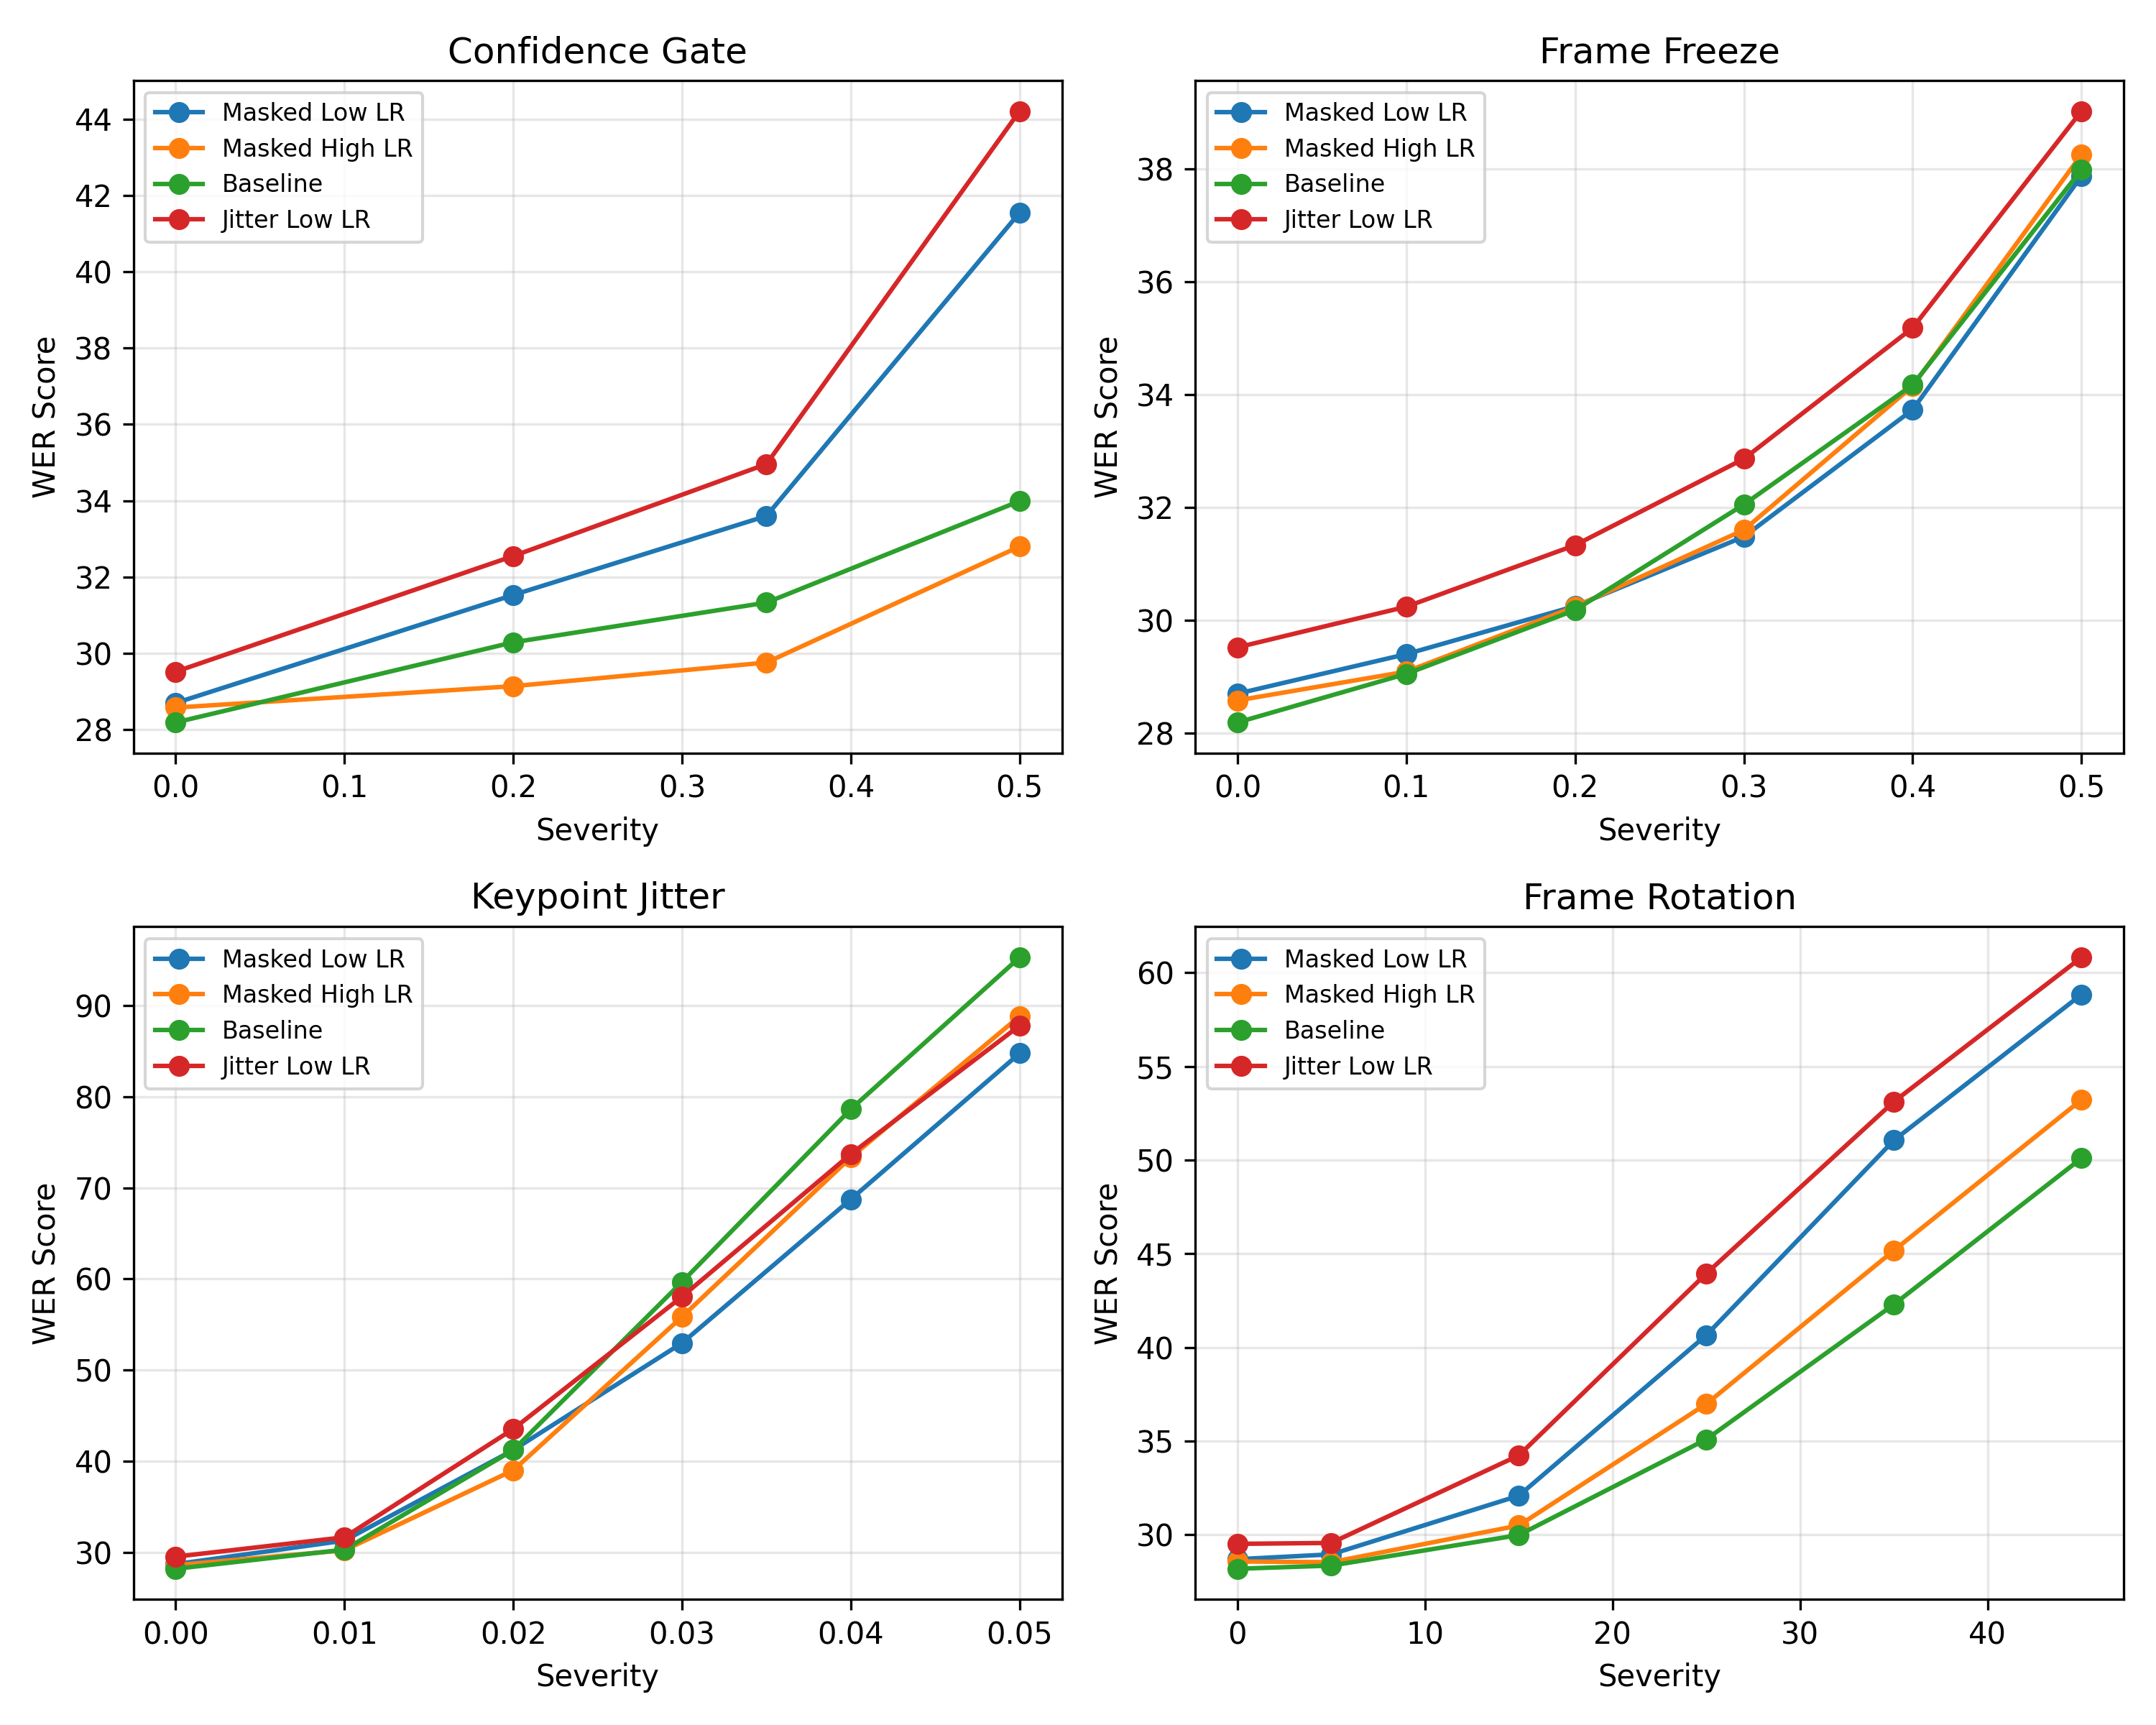
\includegraphics[width=\linewidth]{robustness.png}
  \caption{Model robustness under increasing corruption severities}
  \label{fig:robustness}
\end{figure}


\subsection{Probe and Fine Tune Results}
When examining the results of the probe after pre-training (Table \ref{tab:probe-percent} and Table \ref{tab:probe-masking}), there is a clear separation between the score of the fine-tuned encoder and the score of the randomly initialised encoder. There is a large amount of  noise in the score for all other results and when compared with the random initialised encoder, this shows that it is unclear whether the pre-training had an effect on the ability of the encoder to identify signs. The examination of the probe using the fine tuned encoder showed that the encoder was a valid tool for measuring encoder understanding of sign language patterns. The study of varying pre-training data (Table \ref{tab:probe-percent}) and the ablation study of the corruption techniques (Table \ref{tab:probe-masking}) during pre-training show WER scores fall within a small range that was not significantly different to random. 

There was significant noise within these results with the encoder training on 4\% of pre-training data having a higher WER when compared to similar percentages. Whilst the pre-training of encoder saw a slight improvement as larger percentages of the pre-training data were used, the significance of noise within this was unclear. Examining the logs of the training process, it appeared that pre-training the performance peaked at 2000-2500 steps on a batch size of 10 before the validation score separated from the train score and slowly increased. 20k-25k clips is approximately 3\% of the total (around 750k clips) CSL-News dataset clips, and so training with larger percentages of the dataset is unlikely to have any impact on the performance. Whilst the high jitter and default masking WER scores were lowest, the noise in the scores give no reason to believe that these encoders will have a higher performance. The WER score of the fine-tune encoder gives confidence that the probe can be trained, but the scores of the probe for pre-trained encoders give no indication of their performance after fine tuning.

In Table \ref{tab:fine-tune-models} all four fine tune models WER scores fall within a small variance, it is not clear whether pre-training significantly hurt or aided SLR performance. The only model which had a change from the baseline was the jitter pre-trained fine tune model which performed slightly worse than the baseline at around 1.3 difference. Pre-training may have hurt this model's performance. This aligns with the probe being unable to find any discernible impact from pre-training when examining the model accuracy. 

This null result is not simply due to poor masking configuration as many masking options were explored and analysed independently without significant improvement to the WER score objective over the random encoder. The null result is also unlikely to be due to poor hyper-parameter selection as the different approaches to using the learning rate across the encoder had no discernible effect on the WER scores or predictions. 

\subsection{Prediction analysis}
The pre-trained models show no improvement on performance when compared to the baseline model. Examining the WER score of the individual predictions across the fine tuned models, the pre-trained models correlate strongly with the baseline model (Table \ref{tab:fine-tune-preds}). They appear to fail on the same clips and this appears to be a genuine lack of change in the models rather than just measurement noise. The p-score of 0.227 and 0.137 for the two masked pre-trained models when compared with the baseline using the paired t-test based on the distribution of the WER scores found no statistically significant difference. The jitter pre-trained model showed statistically significant difference for the two-sample t-test but with a negative WER score for improvement when compared with the baseline. 

\subsection{Robustness}
The study identified changes to the robustness of the fine tuned models; these changes were not uniform robustness improvements against the baseline but were shifts in the pattern of model robustness to differing corruptions (Figure \ref{fig:robustness}). The corruptions used for the robustness testing were all unseen by all models aside from the jitter corruption which was used as part of the pre-training for the jitter Low LR model. The study showed the degradation of all models as the severity of the corruption was increased across all corruptions. When examining the differing behaviour between models, the baseline model only showed worse performance than other models for the jitter corruption when the severity was high (over 0.02) (Table \ref{tab:jitter-corruption}). However at this level of corruption (0.03 and higher jitter) all models have such low performance that their usefulness for sign language translation is low. 

 The frame freeze corruption saw uniform robustness across all models (Table \ref{tab:freeze-corruption}). The duplication of individual frames can also be seen as losing frames, the RTMPose dataset was already reduced in frame length by half and this had negligible effect on the performance. The two models with high learning rate appear to perform similarly across the confidence gate and rotation corruptions with higher performance than the low learning rate models (Table \ref{tab:conf-corruption} and Table \ref{tab:rotate-corruption}). The effect of the pre-training in the robustness of the models is unclear due to the similar behaviour of the baseline and the Masked High LR model. 

The single difference between Jitter Low LR and Masked Low LR models was the jitter corruption during pre-training. The jitter model performs moderately worse on all robustness and accuracy tests. When examining the scale of the jitter used during pre-training it aligns with the jitter that caused the Baseline model to score WER of 95.30 in the robustness test. Such a low score suggests that this level of jitter is too high for the model to learn meaningful sign language patterns in the noisy data during pre-training and may account for the poor performance of the jitter model. 

\subsection{Objective Alignment}
The original naive target of the joint positions allowed the model to find a trivial solution. The addition of the velocity saw improvements and was established for skeleton action recognition \cite{shi_decoupled_2020}, but this target may still have been too weak. Whilst generative learning was effective in Uni-Sign, the pre-training target aligned closely with the objective of SLT. Contrastive pre-training seen in SHuBERT learns by discriminating between clusters of sign movements, this appears to align closely with the representation required to discriminate between different gloss signs \cite{hsu_hubert_2021} \cite{liu_self-supervised_2021}. The contrastive approach seen in ShuBERT requires larger datasets and is seed dependent; this approach has no guarantee to produce clusters which align to features relating to textual knowledge. Contrastive pre-training may produce improved performance, but the generative, velocity based approach was a valid path worth investigating cheaply before the contrastive approach is analysed at a larger scale.

\newpage

\section{Conclusion}
\subsection{Contributions and project aims}
The study found that masked keypoint pre-training with a velocity and position was not able to create statistically significant improvements to sign language recognition for the CSL-Daily dataset, when compared with a baseline produced by the MSKA model using the RTMPose pose estimator. Pre-training with masking as well as keypoint jitter produced a statistically significant degradation in the Sign Language Recognition. The pre-trained models showed high correlation with the baseline showing that they largely exhibited the same behaviour across test clips. The linear probe was able to distinguish a large difference performance of the encoder when it was fine tuned, but was unable to distinguish significant differences with the performance when it was pre-trained using a variety of masking methods. The RTMPose pose estimator at half standard frame rate could be used to produce comparable results to the HRNet pose estimator with the MSKA model. The robustness to corruptions of the pre-trained models were not overall improved but were reshaped, causing the model to show increased robustness to some corruptions such as jitter but decreased robustness to corruption in rotation to the viewpoint and gating keypoints by confidence. The project's aim of improving robustness and accuracy overall could not be met, but the robustness was reshaped. The project showed that pre-training could be used to reshape robustness to corruption.

\subsection{Limitations}
The fine tuning was based upon a limited training seed and repeated runs could have shown the scale of the variance of the WER. Without the variance the understanding of the differences between the WER scores are limited, although the analysis of the predictions partially mitigates this. 

Whilst the pre-training was limited to just 20\% of the CSL-News dataset, the model never utilised more than 3\% of the dataset, this may have been a limiting factor if the pre-training did not reach a plateau on such as small subset of the data. 

The corruptions and their severities were constructed rather than derived from measuring the results of pose estimators when the original video was exposed to noise. The original videos could have been exposed to synthetic corruptions before the keypoints were extracted, but this still may not have represented real-world corruptions. The results observed for the robustness study must be caveated as the model's response to synthetic noise instead of measured real-world corruptions.

\subsection{Future Plans}
The fine tuning should be run on many seeds to identify the variance, so that the scale of the WER difference can be understood.
The corruption suite should be grounded in pose estimation run upon corrupted video to identify genuine pose estimator failures. This would allow validation of more genuine corruptions as well all analysis of model robustness to corruptions when trained with genuine corruptions or synthetic corruptions.
Provided the pre-training can be performed on a larger dataset before the validation set diverges, the scale of the pre-training should be extended beyond the 20\% of the CSL-News dataset. There are a large variety of sign language datasets which could be used and the possibility of multi language signing has been established by Uni-Sign. Contrastive pre-training should be investigated as an alternative approach to the generative pre-training used in this project.


\bibliographystyle{IEEEtran} 
\bibliography{MSKA} 

\newpage

% BEGIN APPENDIX
\appendix
\section{Access to code}

The code written for this study can be found here here: \url{https://github.com/wpitt3/SLR_xe25973}

The MSKA project code can be found here: \url{https://github.com/sutwangyan/MSKA}

% \section{Glossary}
% TODO Glossary

\end{document}


